\documentclass[a4paper,11pt, twoside]{article}

\usepackage[a4paper,top=3cm,bottom=3.5cm,left=2.5cm,right=2.5cm]{geometry}
\usepackage{graphicx}
\usepackage[utf8x]{inputenc}
\usepackage[italian]{babel}
\usepackage{fancyhdr}
\usepackage{amssymb}
\usepackage{makeidx}
\usepackage{eurosym}
\usepackage{hyperref}
\usepackage{varioref}
\usepackage{xmpincl}
\usepackage{ccicons}
\usepackage{listings}
\usepackage{color}
\usepackage{subfigure}

%\usepackage{microtype}


\usepackage{amsthm}

\theoremstyle{definition}
\newtheorem{defn}{Definizione}[section]

\addto\captionsitalian{%
\renewcommand{\lstlistingname}{Codice}}
\lstloadlanguages{[ANSI]C,Java}

\title{Appunti di Sistemi Distribuiti}
\author{Matteo Gianello}
\date{\today}

\pdfinfo{%
  /Title    (Appunti di Sistemi Distribuiti)
  /Author   (Matteo Gianello)
  /Creator  (Matteo Gianello)
  /Producer ()
  /Subject  ()
  /Keywords (Sistemi Distribuiti Cugola IngInf Polimi)
}
\makeindex
\includexmp{licenza}

\lstset{basicstyle=\small\ttfamily,
keywordstyle=\color{blue}\bfseries,
commentstyle=\color{green},
stringstyle=\color{red},
showstringspaces=true,
numbers=left,
frame=single,
columns=fullflexible,
breaklines=true,
float=tb,
captionpos=b}

\begin{document}
\pagestyle{empty}
\thispagestyle{empty}
\maketitle
\vspace{5cm}
\begin{center}
Quest'opera è stata rilasciata con licenza Creative Commons Attribuzione - Non commerciale - Condividi allo stesso modo 3.0 Unported. Per leggere una copia della licenza visita il sito web \url{http://creativecommons.org/licenses/by-nc-sa/3.0/deed.it} \ccbyncsa.
\end{center}
\newpage

\thispagestyle{plain}
\tableofcontents
\newpage

\pagestyle{plain}
\label{capitolo1}
\section{Introduzione}
A partire dalla metà degli anni '80, grazie a due innovazioni tecnologiche si fecero diversi passi avanti nell'uso dei calcolatori. La prima di queste innovazioni fu lo sviluppo di microprocessori potenti; la seconda grande innovazione fu l'invenzione delle reti di computer con l'introduzione delle \textbf{LAN} (\emph{Local Area Network}) che consentirono a centinaia di macchine di essere connesse le une alle altre e permisero lo scambio di piccole quantità di informazioni in pochi microsecondi.\\
Il risultato di questa innovazione tecnologica è che oggi mettere insieme una grande quantità di computer tramite una rete ad alta velocità è diventato molto semplice. Questo tipo di sistemi sono solitamente chiamate \emph{reti di computer} o \textbf{sistemi distribuiti}.
\subsection{Definizione di sistema distribuito}
Esistono diverse definizioni di \emph{Sistema distribuito} ma tutte quante sono abbastanza insoddisfacenti. Daremo ora una prima definizione che è sufficente per i nostri scopi:
\begin{center}
\emph{Un sistema distribuito è una collezione di computer indipendenti che appare ai propri utenti come un singolo sistema coerente}
\end{center}
Da questa definizione possiamo ricavare diversi caratteristiche di un sistema distribuito, la prima è che i sistemi distribuiti sono costituiti da componenti autonomi; la seconda è che gli utenti, siano essi persone o altri programmi, vedono il sistema come un'unica entità. Il che significa che i diversi componenti devono in qualche modo collaborare.\\
Quello che non viene specificato in questa definizione è il tipo di computer usati per i componenti ne come questi sono interconnessi.\\
Le caratteristiche più importanti dei sistemi distribuiti sono il fatto che le differenze tra i vari computer e le loro modalità di comunicazione risultano per lo più nascoste agli utenti finali. Inoltre gli utenti possono interagire con un sistema distribuito in modo \emph{consistente} e \emph{uniforme} ovvero indipendentemente da dove e quando avviene l'interazione.\\
Teoricamente i sistemi distribuiti dovrebbero essere facilmente espandibili e scalabili, inoltre, i sistemi distribuiti sono di norma sempre disponibili anche se alcune sui parti sono momentaneamente fuori uso.\\
Allo scopo di supportare reti eterogenee e sistemi operativi differenti alle volte si introduce uno strato software tra lo strato di applicazione e i diversi sistemi operativi, questo strato è chiamato \textbf{middleware} come mostrato in figura \ref{fig:midd}.
\begin{figure}[htb]
\centering
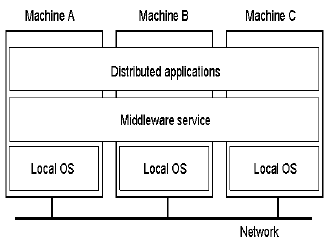
\includegraphics[width=8cm]{img/schemamidd.png}\\
\label{fig:midd}
\caption{Schema di un middleware}
\end{figure}
\subsection{Obiettivi}
La possibilità costruire sistemi distribuiti non implica che tutti i sistemi debbano essere costruiti come sistemi distribuiti. Per far si che sia utile progettare e costruire un sistema distribuito dobbiamo rispettare alcune caratteristiche. un sistema distribuito dovrebbe:
\begin{itemize}
\item rendere le risorse facilmente accessibili,
\item nascondere il fatto che le risorse sono distribuite sulla rete,
\item essere aperto,
\item essere scalabile.
\end{itemize}
\subsubsection{Accessibilità delle risorse}
L'obiettivo principale di un sistema distribuito è quello di rendere facile l'accesso alle risorse remote e condividerle in maniera efficiente e controllata.\\
Ma che cosa intendiamo per "risorse"? Con il termine \emph{risorse} possiamo indicare qualsiasi cosa, alcuni esempi tipici sono stampanti, computer, dati, file, pagine web o intere reti.
Le ragioni che portano a voler condividere le risorse sono molteplici, la prima è sicuramente quella economica, pensiamo ad esempio a ricercatori che condividono un supercomputer o ad una stampante condivisa in un ufficio. Inoltre, la connessione di più utenti facilita la collaborazione come avviene nei \textbf{groupware} dove gruppi di persone lavorano insieme anche stando in diverse parti del mondo.\\
Tutto questo incremento di connessione e collaborazione dovrebbe portare però ad una necessaria crescita anche in termini di sicurezza, anche se nella pratica attuale tale incremento nei sistemi di sicurezza non è ancora avvenuto; non è raro trovare sistemi in cui password e altre informazioni sensibili sono inviate come testo in chiaro. Altri problemi legati alla sicurezza sono l'aumento delle \emph{junk mail} o mail di \emph{spam} e l'invio e la raccolta di informazioni riguardanti l'utente per creare un profilo mentre è connesso.
\subsubsection{Trasparenza}
Uno degli obiettivi principali in  un sistema distribuito è quello di nascondere che i processi e le risorse sono distribuiti. Un sistema in grado di presentarsi come un singolo computer è detto \textbf{trasparente}.\\
Possiamo catalogare la trasparenza in diversi tipi in quanto qesto concetto può riguardare molti aspetti di un sistema distribuito.\\
La \textbf{trasparenza all'accesso} riguarda le differenze nella rappresentazione dei dati e la modalità di accesso alle risorse da parte degli utenti. Ovvero si desidera nascondere le differenze nelle macchine e trovare un accordo nella rappresentazione dei dati.
Un altro importante tipo di trasparenza è la \textbf{trasparenza di ubicazione} che si prefigge l'obiettivo di nascondere agli utenti la localizzazione di una risorsa. I \emph{nomi} in questa tipo di trasparenza giocano un ruolo importante in quanto è possibile raggiungere tale trasparenza assegnando ad ogni risorsa un nome logico indipendente dalla sua locazione, un esempio di tale tecnica sono gli \emph{URL}.\\
Alcuni sistemi distribuiti che consentono lo spostamento delle risorse senza compromettere la possibilità di accesso devono fornire la \textbf{trasparenza alla migrazione}. Nel caso in cui le risorse possono essere spostate \emph{durante} l'utilizzo senza che utenti o applicazioni notino tale spostamento si deve garantire anche la \textbf{trasparenza al riposizionamento}.\\
La \textbf{trasparenza alla replica} riguarda la possibilità di fornire una o più copie della stessa risorsa per aumentarne la disponibilità e migliorare le prestazioni, tutto questo nascondendo all'utente il fatto che la risorsa è replicata.\\
Come già detto l'obiettivo principale dei sistemi distribuiti è la condivisione di risorse, ma questa porta in alcuni casi ad avere una condivisione di tipo \emph{competitivo} ovvero, più utenti vorrebero accedere alle stesse risorse (es. una tabella di un database) tutto ciò deve essere evitato tramite la \textbf{trasparenza alla concorrenza} che deve lasciare la risorsa in uno stato consistente. Questa consistenza può essere ottenuta tramite diverse meccanismi tra cui ad esempio il \emph{locking} nel quale gli utenti ottengono a turno l'accesso esclusivo ad una risorsa.\\
Per introdurre l'ultimo tipo di concorrenza partiamo da un'altra definizione di sistema distribuito
\begin{center}
\emph{Ne apprendi l'esistenza quando il crash di un computer di cui non hai mai sentito parlare ti impedisce di portare a termine qualunque lavoro}
\end{center}
Questa definizione pone un altro aspetto importante della progettazione di un sistema distribuito, quello della gestione dei guasti; rendere un sistema \textbf{trasparente ai guasti} significa far si che un utente non si renda conto che una risorsa smette di funzionare correttamente. La difficoltà più grande è distinguere quando una risorsa è morta da quando è semplicemente molto lenta.\\
Sebbene in generale si preferisce avere sistemi trasparenti ci sono situazioni in cui nascondere completamente agli utenti la distribuzione del sistema non è una buona idea. Come nel caso si voglia contattare un servizio che sta dall'altra parte del mondo e si voglia una risposta in un tempo inferiore ai 35ms; o quando si vuole che due repliche siano sempre consistenti, nel caso di server in due continenti diversi un aggiornamento potrebbe richiedere alcuni secondi.\\
Il problema principale che limita però la trasparenza è la trasparenza stessa, infatti, ammettendo che la completa trasparenza di un sistema è \emph{impossibile} è \emph{saggio} cerca di ottenerla a tutti i costi? Rendere la distribuzione esplicita può aiutare gli utenti a capire eventuali comportamenti \emph{anomali} del sistema.
\subsubsection{Apertura}
un altro obiettivo dei sistemi distribuiti è l'apertura. un sistema distribuito \textbf{aperto} è un sistema che offre servizi rispettando delle regole standar che descrivono la sintassi e la semantica dei servizi stessi.\\
Nei sistemi distribuiti i servizi sono descritti tramite \textbf{interfacce} per lo più utilizzando un linguaggio denominato \emph{IDL (interface description language)} che però descrive soltanto la sintassi delle interfacce, ovvero, il nome delle funzioni e i tipi di parametri, i valori di ritorno o le possibili eccezioni sollevate. Per la descrizione di che cosa fa il servizio, invece, si usa solitamente il linguaggio naturale.\\
Se l'interfaccia è ben specificata un processo che ha bisogno di una determinata interfaccia può comunicare con un altro processo che implementa tale interfaccia; inoltre, consente a due processi distinti di implementare tale interfaccia in due modi completamente diversi, il che porta a due sistemi distribuiti che però  operano allo stesso modo.\\
Una specifica però deve essere \emph{completa} e \emph{neutrale}, completa significa che viene specificato tutto ciò che è necessario per realizzare un'implementazione, ma ottenere la completezza è molto difficile e perciò di solito un programmatore deve aggiungere dettagli specifici dell'implementazione. Per neutrale si intende, invece, che la specifica non deve imporre dettagli sull'implementazione. Completezza e neutralità portano ad altre due importanti caratteristiche che i sistemi distribuiti dovrebbero soddisfare, \textbf{interoperabilità} che significa che due implementazioni di vendor diversi possono collaborare e coesistere basandosi unicamente su di uno standar comune. \textbf{Portabilità} indica la possibilità di eseguire un applicazione scritta per un sistema distribuito $A$ su di un sistema distribuito $B$ senza dover apportare modifiche all'applicazione.\\
Infine un altro obiettivo che i sistemi distribuiti dovrebbero prefissarsi è che l'aggiunta o la sostituzione di componenti dovrebbe risultare facile e non influire sui componenti già presenti; questa caratteristica sta ad indicare che il sistema distribuito è \textbf{ampliabile}.
Per ottenere la flessibilità in un sistema aperto è fondamentale che esso sia organizzato come un insieme di componenti piccolo e e facilmente sostituibile e adattabile. Ma questo comporta fornire le interfacce non solo dei componenti che si interfacciano direttamente con gli utenti ma anche dei componenti interni.
\subsubsection{Scalabilità}
La scalabilità sta diventando uno degli aspetti più importanti dei sistemi distribuiti a causa della grande diffusione di internet. Esistono diversi tipi di scalabilità la prima si ha quando un sistema è scalabile rispetto alla sua dimensione il che significa che possiamo aggiungere utenti e risorse. Un sistema può essere scalabile geograficamente quando utenti e risorse sono situati in luoghi molto lontani.
Ed, infine, un sistema può essere scalabile anche dal punto di vista dell'amministrazione ovvero quando comprende molte infrastrutture indipendenti rimane comunque facile da gestire.\\
La scalabilità richiede di affrontare molti problemi. Prendiamo ad esempio la scalabilità rispetto alla dimensione, alcuni servizi in un sistema distribuito possono essere forniti da un unico server questo fa si che aggiungendo utenti quel particolare server diventa un collo di bottiglia per l'intero sistema. A volte l'uso di un solo server è inevitabile come nel caso della gestione di dati sensibili.
Per quanto riguarda la scalabilità a livello geografico anch'essa comporta innumerevoli problemi, infatti, la maggior parte dei sistemi distribuiti che lavorano su LAN si basano sulla comunicazione \textbf{sincrona} nella quale un \emph{client} richiede una risorsa e resta in attesa che tale risorsa sia disponibile. Questo meccanismo non è applicabile per sistemi globali nei quali la comunicazione tra due computer può richiedere anche qualceh millisecondo. In oltre si deve tener conto che la comunicazione su WAN(\emph{wide area network}) è inaffidabile e praticamente sempre punto a punto (\emph{pont-to-point}). Al contrario le reti locali più affidabili permettono anche il \emph{broadcasting} ovvero l'invio simultaneo a tutte le macchine delle rete dello stesso messaggio.\\
Dopo aver visto i problemi di scalabilità ci chiediamo come risolvere tali problemi nei sistemi distribuiti.
\section{Architetture}\label{capitolo2}
I sistemi distribuiti sono spesso definibili come pezzi di software sparsi su molte macchine. Al fine di dominare la loro complessità è necessario che questi sistemi siano organizzati. Un modo semplice per distinguere l'organizzazione di un sistema distribuito, è quello di distinguere l'organizzazione logica dei componenti software e la relativa realizzazione fisica.\\
Per \emph{architetture software} intendiamo l'organizzazione e l'interazione dei vari componenti software; mentre l'effettiva realizzazione di un sistema distribuito richiede che i componenti software siano istanziati su macchine reali, l'architettura risultante viene detta \emph{architettura di sistema}.Analizzeremo per prime le architetture centralizzate in cui un server implementa la maggior parte delle funzionimentre client remoti accedono al server tramite semplici mezzi di comunicazione.\\
\subsection{Stili architetturali}
Iniziamo l'analisi dalle diverse tipologie di architetture software in quanto progettazione e adozione di una adeguata architettura sono fondamentali per la riuscita e la manuntenibilità del sistema.\\
Introduciamo ora la nozione di \emph{stile architetturale} che esprime in termini di componenti mezzi di comunicazione e messaggi scambiati. Un \emph{componente} è un'unità modulare con interfacce ben definite e sostituibile nel suo ambiente.\\
La comunicazione tra i diversi componenti avviene tramite quello che è definito \emph{connettore} ovvero un sistema che implementa le chiamate a procedure remote piuttosto che il passaggio di messaggi o lo streaming dei dati.\\
Usando componenti e connettori possiamo ottenere diverse configurazioni che a loro volta sono classificati in diversi \emph{stili architetturali}. I più importanti stili architetturali ad oggi identificati sono:
\begin{itemize}
\item architettura a livelli (\emph{layer})
\item architetture basate sugli oggetti
\item architetture centrate sui dati
\item architetture basate sugli eventi
\end{itemize}
Per quanto riguarda lo stile a livelli è quello più semplice nel quale i componenti sono organizzati a strati in cui un componente del livello $L_i$ può chiamare un componente del livello $L_{i-1}$ ma non può contattare i componenti dello stesso livello. Questo modello è uno dei più utilizzati nelle applicazioni di rete, le richieste scendono lungo la catena gerarchica mentre le risposte risalgono.\\
Le \emph{architetture basate sugli oggetti} hanno un organizzazione meno rigida, ogni oggetto corrisponde ad un componente e tutti gli oggetti sono connessi tramite \emph{chiamate a procedura remota}; questo tipo di architettura corrisponde esattamente al caso client-server ed insieme a quella a livelli costituiscono il 90\% delle architetture dei sistemi distribuiti presenti oggi.\\
Le \emph{architetture basate sui dati} si sviluppano attorno all'idea che i processi comunicano attraverso un \emph{repository} comune.\\
Nelle \emph{architetture basate sugli eventi} i processi comunicano essenzialmente attraverso la propagazione degli eventi, i più noti tipi di sistemi distribuiti che utilizzano la propagazione degli eventi sono i sistemi \emph{publish/subscribe} nei quali alcuni processi pubblicano degli eventi ed è il middleware ad assicurarsi che questi eventi siano ricevuti soltanto da qui processi che si sono iscritti a quel determinato evento.\\
Nel caso in cui si combinino le architetture basate sugli eventi con quelle basate sui dati si ottiene una architettura chiamata \emph{spazio di dati condivisi} che permette ai processi di essere disaccoppiati anche nel tempo in quanto non è necessario che i processi siano attivi nell'istante in cui avviene la comunicazione.
\subsection{Architetture di sistema}
Abbiamo visto fino ad ora alcune scelte architetturali, vediamo ora come sono effettivamente organizzati la maggior parte dei sistemi distribuiti considerando dove sono posizionati i componenti software. La scelta di quali componenti usare e di come posizionarli porta alla realizzazione della cosiddetta \emph{architettura di sistema}.
\subsection{Architetture centralizzate}
La prima architettura che analizzeremo è quella \emph{centralizzata}, in quanto pensare ad un sistema in termini di \emph{client} che richiedono dei servizi a dei \emph{server} facilita la comprensione e la gestione dei sistemi distribuiti.\\
Nel modello client-server i processi sono suddivisi in due gruppi; un \textbf{server} è un processo che implementa uno specifico servizio. Un \textbf{client} è invece un processo che richiede un servizio ad un serve inviandogli una richiesta e quindi attendendo una risposta.\\
La comunicazione tra client e server può essere implementata per mezzo di un semplice protocollo senza connessione quando la rete sottostante è molto affidabile. In questo caso quando un client richiede un servizio invia un messaggio al server indicando il servizio richiesto e i dati di input. Quest'ultimo all'arrivo della richiesta la processa e confeziona i risultati in un altro messaggio.\\
L'utilizzo di un protocollo senza connessione ha il vantaggio di essere efficiente fino a quando non abbiamo perdita di pacchetti. Si potrebbe pensare di impostare il client affinché rinvii il messaggio quando non riceve alcuna rsposta, ma non si può stabilire se è stato perso il messaggio o la risposta e quindi il server ha compiuto oppure no l'operazione richiesta. In alcuni casi le richieste sono \emph{idempotenti} ovvero possono essere ripetute senza danni.\\
Per risolvere il problema della perdita di messaggi, molte architetture client-server utilizzano dei protocolli affidabili orientati alla connessione.
\paragraph{Stratifficazioni delle applicazioni}
Il problema principale dell'architettura client server è che non vi è una netta distinzione tra quali sono le funzionalità del client e quelle del server; è stata così introdotta una un nuovo tipo di suddivisione delle diverse funzionalità in base che esse siano più vicine all'utente o ai dati. I tre livelli identificati sono:
\begin{itemize}
\item il livello dell'interfaccia utente
\item il livello applicativo
\item il livello dei dati
\end{itemize}
Il livello dell'interfaccia utente contiene tutto ciò che è necessario per interfacciarsi con l'utente come la gestione della grafica. Il livello applicativo di solito contiene le applicazioni. Il livello dei dati gestisce tutto ciò che concerne i dati da gestire.\\
Esistono diversi modi in cui questi tre livelli possono essere istanziati sull'hardware come possiamo vedere in \figurename~\ref{fig:layer}.
La configurazione più utilizzata è quella nel quale il client implementa solo il livello dell'interfaccia utente (\emph{thin client}) ma esistono altri sistemi una parte dal livello applicativo si trova implementata nel client, in questo caso si parla di \emph{fat client}.
\begin{figure}[htb]
\centering
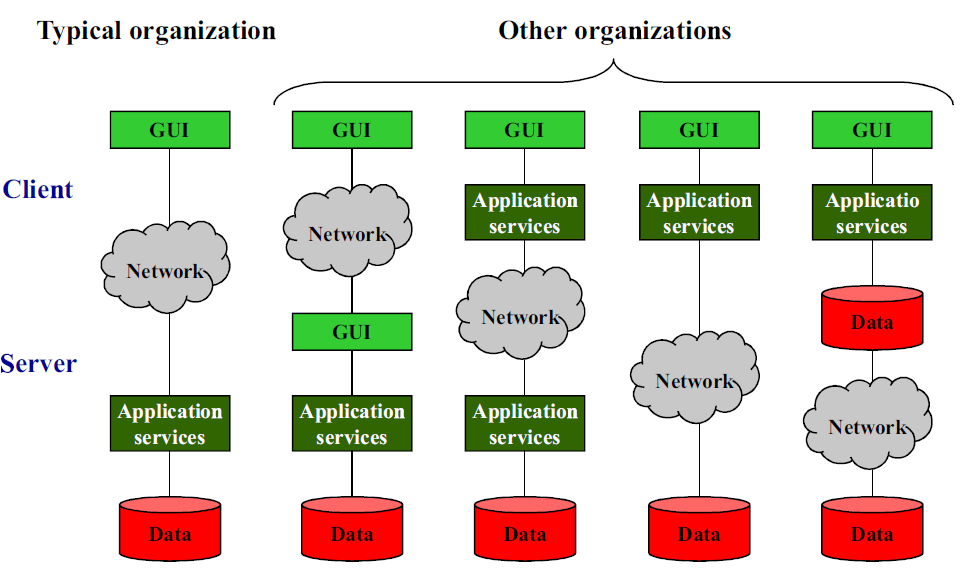
\includegraphics[width=8cm]{img/layer.png}\\
\caption{Esempio di suddivisione dei layer}\label{fig:layer}
\end{figure}
Per quanto riguarda il livello dei dati molte volte è gestito da meccanismi che rendono i dati \textbf{persistenti} anche quando non vi sono altre applicazioni in esecuzione. In alcuni casi molto semplici il livello dei dati consiste in un  \emph{filesystem} ma nella maggioranza dei casi si tratta di una \emph{base di dati}
\paragraph{Architetture multi livello}
La suddivisione delle applicazioni in tre livelli logici suggerisce anche una distribuzione fisica delle applicazioni client serversu molte macchine, la distribuzione più semplice è quella su due macchine:
\begin{enumerate}
\item una macchina client che contiene solo i programmi dell'interfaccia utente
\item una macchina server contenete il resto dei programmi e i dati
\end{enumerate}
Si possono suddividere le applicazioni anche in altri modi come visto in \figurename~\ref{fig:layer}.\\
La tendenza degli ultimi anni è quella di suddividere i diversi livelli su più macchine in modo da creare una architetture multi livello.
Un esempio pratico ad esempio è quello mostrato in \figurename~\ref{fig:3layer} nella quale si mostra un architettura a 3 livelli.\\
\begin{figure}[htb]
\centering
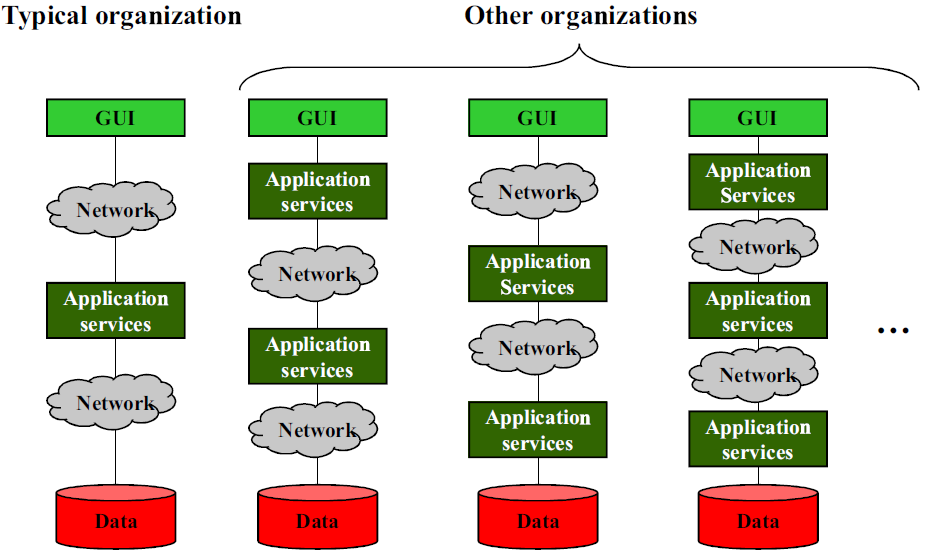
\includegraphics[width=8cm]{img/3layer.png}
\caption{Esempio di suddivisione dei layer su 3 livelli}\label{fig:3layer}
\end{figure}
\subsubsection{Architetture decentralizzate}
La suddivisione delle architetture client server in livelli denota un tipo di distrinuzione detta \emph{verticale} in quanto i componenti sono divisi su più macchine seguendo un criterio \emph{logico}.\\
Questo tipo di distribuzione è utile con le architetture client-server ma nel caso in cui la distribuzione che conta è quella dei client e dei server e non delle funzioni allora si parla di \emph{frammentazione orizzontale}. Un esempio molto conosciuto di architettura con distribuzione orizzontale sono i \textbf{sistemi peer-to-peer}.\\
I processi che costituiscono un sistema peer-to-peer sono tutti uguali, di conseguenza l'interazione tra processi è quasi del tutto simmetrica e i processi agiscono sia da client che da server e per questo sono anche detti \textbf{servent}.\\
Dato questo tipo di comportamento il problema principale delle reti \emph{p2p} è quello di organizzare i processi in una rete \emph{overlay} ovvero una rete nella quale i processi costituiscono i nodi e i collegamenti rappresentano i canali di comunicazione. Con questa struttura un processo non può comunicare direttamente con un altro processo arbitrario ma deve seguire i canali di comunicazione disponibili.\\
Esistono due tipi principali di reti \emph{overlay} quelle strutturate e quelle non strutturate.
\paragraph{Architetture peer-to-peer strutturate}
In una rete p2p strutturata la rete overlay è costruita usando una procedura deterministica, quella più comune è l'uso di una \textbf{hash tabel distribuita} (DHT). In questo tipo di struttura ai dati viene assegnato un identificatore univoco in uno spazio molto grande (129:160 bit). Anche ai nodi del sistema viene assegnato un identificatore nello stesso spazio dei dati. Il punto cruciale di questa architettura è quello di creare uno schema efficiente e deterministico che associ univocamente la chiave di un dato con l'identificativo di un nodo basandosi su un'opportuna metrica di distanza. Inoltre, è importante che quando si effettua la ricerca di un dato sia restituito l'indirizzo del nodo al quale questo dato è associato, e ciò si ottiene \emph{instradando} la richiesta al nodo associato.\\
Ad esempio nel sistema \emph{Chord} i nodi sono organizzati logicamente ad anello, ed i dati sono organizzati assegnando i dati con identificativo $k$ al nodo con più piccolo identificativo $id>k$; questo nodo è chiamato \emph{successore} della chiave $k$ ed è identificato come $succ(k)$ come mostrato in \figurename~\ref{fig:chordring}.\\
\begin{figure}[htb]
\centering
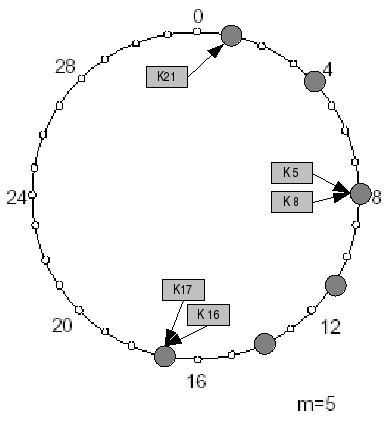
\includegraphics[width=8cm]{img/chordring.jpg}\\
\caption{Esempio di sistema Chord}\label{fig:chordring}
\end{figure}
La parte più importante della gestione di una rete overlay strutturata è la \textbf{gestione dell'appartenenza} da parte dei nodi. Quando un nodo vuole unirsi alla rete genera un \emph{id} casuale ed effettua una ricerca di $id$ a questo punto il sistema restituirà $succ(id)$. Alla fine per inserirsi il nuovo nodo contatterà il successore individuato dalla ricerca e il suo predecessore e si inserirà nell'anello. Inoltre, l'inserimento causa la migrazione dei dati associati ad $id$ da $succ(id)$.
L'uscita è molto semplice il nodo informa della sua dipartita il $succ(id)$ e il suo predecessore e trasferisce i dati a $succ(id)$.\\
\paragraph{Architetture peer-to-peer non strutturate}
I sistemi peer-to-peer non strutturati si basano su algoritmi casuali per costruire la rete \emph{overlay}. L'idea è quella che ogni nodo mantenga una lista dei suoi vicini. Inoltre, anche i dati sono posizionati sui nodi in modo casuale, di conseguenza l'unico modo di effettuare una ricerca è inoltrare la richiesta a tutta la rete.\\
L'obiettivo principale di un sistema p2p non strutturato è la creazione di un \textbf{grafo disordinato}. Per fare ciò ogni nodo mantiene una lista di $c$ vicini scelti a caso dall'insieme dei nodi \emph{vivi}; questa vista è detta \textbf{vista parziale}.
Ora supponiamo che un nodo voglia aggiungersi alla rete, esso contatta in altro nodo arbitrario dalla lista dei punti di accesso; questo punto di accesso è un normale nodo della rete che però ha un alta probabilità di essere disponibile. I meccanismi che creano la rete overlay sono detti \emph{push} e \emph{pull} e permettono lo scambio delle informazioni per la costruzione della rete tra i nodi. Questi meccanismi usati singolarmente possono portare alla creazione di reti overlay disconnesse, per questo si usano entrambe le tecniche.\\
L'uscita dalla rete è molto semplice, infatti, visto che i nodi si scambiano periodicamente le viste parziali basta solo che il nodo lasci la rete, gli altri nodi con il passare del tempo si accorgono dell'assenza del nodo che ha lasciato la rete e lo elimina dalla sua vista parziale.
\paragraph{Gestione della topologia di una rete overlay}
Anche se i sistemi p2p strutturati e non strutturati sembrano costruire due classi completamente diverse, in realtà selezionando attentamente gli elementi scambiati nelle viste parziali è possibile costruire reti overlay con tipologie specifiche. Un esempio molto interessante sono quelle funzioni che cercano di cogliere la \textbf{vicinanza semantica} dei dati che creano reti \textbf{overlay semantiche} che permettono ricerche efficienti nei sistemi p2p non strutturati.
\paragraph{Superpeer}
Specialmente nelle reti non strutturate al crescere delle dimentsioni potrebbe diventare problematico localizzare i dati. Questo è dovuto al fatto non esiste un modo deterministico per instradare una richiesta di ricerca.\\
Per evitare questo problema molte reti p2p hanno proposto l'utilizzo di nodi speciali che mantengono un indice dei dati. Questo tipo di nodi sono detti \textbf{superpeer}. I superpeer sono organizzati tra loro tramite una rete p2p; si forma così una struttura ad albero. L'accesso ad un normale peer avviene attraverso l'accesso al superpeer.
\subsubsection{Architetture ibride}
Fino ad ora abbiamo visto le architetture centralizzate client-server e alcune architetture peer-to-peer ora vediamo come queste due tipologie di architetture possono combinarsi per dare vita ad altre architetture dette \emph{ibride}
\paragraph{Sistemi edge-server}
I sistemi \emph{edge-server} sono una classe molto diffusa di architetture ibride. In questa classe i server sono posti ai bordi della rete Internet ovvero tra la rete Internet e quelle aziendali come nel caso degli \textbf{Internet service provider}. I client si connettono alla rete internet tramite un edge-server il quale fornisce i contenuti dopo aver applicato dei filtri e funzioni di transcodifica.
\paragraph{Sistemi distribuiti collaborativi}
Le strutture ibride sono largamente utilizzate nei sistemi distribuiti collaborativi dove sono necessarie velocità nell'entrare nel sistema e per questo viene utilizzato uno schema di tipo client-server. Dopo di che si usa uno schema completamente decentralizzato.\\
Un sistema concreto che utilizza questo meccanismo è il sistema \emph{BitTorrent}
\subsection{Architetture e middleware a confronto}
Considerando le questioni architetturali viste fino ad ora ci chiediamo quale ruolo giochi il middleware visto nei capitoli precedenti.\\
Il middleware in realtà costituisce uno strato tra le applicazioni e le piattaforme distribuite ed il suo obiettivo è quello di fornire un certo grado di trasparenza alla distribuzione. Ciò che accade in realtà è che i middleware seguono uno specifico stile architetturale (ad oggetti come \emph{CORBA} o ad eventi come \emph{TIB/Rendezvous}). Avere un middleware basato su di un certo stile architetturale rende più semplice la progettazione e la realizzazione delle applicazioni.\\
Lo svantaggio più grande è però il fatto che un middleware può  non essere ottimale per una determinata applicazione ciò porta ad avere o middleware molto grandi o a diverse versioni per una specifica classe di applicazioni.
\subsubsection{Interceptor}
Concettualmente un \emph{interceptor} non è altro che un costrutto software che interrompe il normale flusso di controllo e consente ad altro codice di essere eseguito. Rendere però un interceptor generico è molto arduo e a volte averne uno con funzionalità limitate migliorerà sia la gestione del software che che il sistema distribuito nel suo complesso.\\
Il concetto è che un oggetto $A$ può richiamare un metodo appartenete all'oggetto $B$ ache se quest'ultimo risiede su una macchina diversa da $A$.
I passi per eseguire questa chiamata remota sono:
\begin{enumerate}
\item All'oggetto $A$ viene fornita un interfaccia locale esattamente uguale a quella fornita dall'oggetto $B$; a questo punto $A$ richiama il metodo disponibile nell'interfaccia
\item La chiamata di $A$ è trasformata in un'invocazione a un oggetto generico disponibile tramite un'interfaccia generale messa a disposizione dal middleware.
\item L'invocazione a questo oggetto generico viene trasformata in un messaggio inviato attraverso l'interfaccia di rete.
\end{enumerate}

\label{capitolo3}
\section{Modelling}
Nel precedente capitolo abbiamo visto il perchè di alcune scelte architetturali nei sistemi distribuiti; in questo capitolo invece analizzeremo alcuni dei modelli esistenti e di come questi siano realmente utilizzati.
\subsection{Architettura service oriented}
Partendo dal concetto di architettura client-server si può pensare di costruire una architettura costruita interamente attorno al concetto di servizio (\emph{service provider, service consumer, service brokers}). Un servizio rappresenta un insieme di funzionalità vagamente legate tra loro che sono messe a disposizione di una unita chiamata \textbf{fornitore di servizi} (\emph{service provider}). Il \textbf{brokers} mantiene la descrizione dei servizi disponibili che possono essere cercati dai \textbf{consumer} che poi li richiamano quando ne hanno bisogno.\\
Con il termine \emph{orchestration} si indicano l'insieme di invocazioni di determinati servizi in un flusso di lavoro per soddisfare un determinato obiettivo.
\subsection{REST style}
Lo stile REST (\emph{REpresentational State Transfert}) è allo stesso tempo un "buon" modo di descrivere il web  e un insieme di principi che definiscono come gli standard del Web dovrebbero essere utilizzati.\\
Gli obiettivi principali del REST includono :
\begin{itemize}
\item La scalabilità delle interazioni tra componenti
\item Generalità delle interfacce
\item Sviluppo indipendente dei componenti
\item Componenti intermedi per ridurre le latenze aumentare la sicurezza ed incapsulare i componenti legacy.
\end{itemize}
Le principali caratteristiche del sistema REST sono che anch'esso è basato su un architettura client-server; le interazioni sono di tipo \emph{stateless}, gli stati devono essere trasferiti di volta in volta dal client al server;.
I dati che giungono come risposta ad una richiesta devono essere etichettati come cacheable oppure non-cacheable; ogni componente non può comunicare con se non con i layer più vicini. I client devono supportare il \emph{code-on-demand}; ed infine, i componenti devono esporre un interfaccia uniforme.\\
Per quanto riguarda l'ultimo punto le interfacce dei componenti devono soddisfare quattro vincoli principali:
\begin{itemize}
\item Tutte le risorse devono essere identificate da un id (solitamente un \emph{URI}) ed ogni risorsa con un id è una risorsa valida
\item Manipolazione delle risorse tramite la loro rappresentazione, i diversi componenti comunicano tramite il trasferimento di rappresentazioni delle risorse in formati standard (XML) selezionati dinamicamente in base alle capacità o alle informazioni desiderate.
\item Messaggi auto-descrittivi, i messaggi contengono al loro interno dei metadati che ne indicano il tipo di richiesta oppure il significato delle risposte. Questa tecnica è utilizzabile per parametrizzare le richieste
\item Link ipermediali, i client cambiano il loro stato attraverso le richieste che avvengono tramite dei link ipermediali.
\end{itemize}
\subsubsection{Peer-to-Peer}
Come visto nel capitolo \ref{capitolo2} nei sistemi peer-to-peer non esistono dei ruoli definiti ma tutti i componendi giocano lo stesso ruolo. Come già detto i sistemi p2p a differenza di quelli client-server permettono di scalare in modo migliore
\subsection{Object oriented}
Nel caso \emph{Object Oriented} i componenti distribuiti incapsulano i dati e permettono l'accesso e la modifica solo tramite un interfaccia messa a disposizione da ogni componente. I diversi componenti interagiscono tramite RPC.
Questo tipo di sistema si basa sul modello p2p ma il più delle volte è utilizzato per implementare meccanismi client-server
\subsection{Data centered}
Nel caso incentrato sui dai i componenti comunicano, solitamente in modo passivo, con un repository centrale nel quale i dati possono essere recuperati o aggiunti. La comunicazione avviene tramite chiamata a procedura remote e l'accesso ai repository è solitamente sincronizzato.
\subsubsection{Il modello Linda}
Il modello Linda è un modello introdotto negli anni '80 ed incentrato sulla condivisione dei dati, tale modello è usato principalmente nei sistemi di calcolo parallelo.\\
In questo modello la comunicazione è persistente e basata sul contesto si ottiene così un alto grado di disaccoppiamento.
Le caratteristiche principali di Linda sono:
\begin{itemize}
\item I dati sono memorizzati in sequenza in base al tipo di campi (\emph{tuple})
\item Le tuple sono memorizzate in uno spazio persistente e globale (\emph{spazio delle tuple})
\item Operazioni standard come \textbf{out}($t$) che scrive le tuple nello spazio delle tuple \textbf{rd}$(p)$ che legge le tuple che coincidono con il pattern $p$ 
\end{itemize}
Il problema principale di questo sistema è che il modello a spazio di tuple non è facilmente scalabile soprattutto quando aumenta l'area del dominio. Il sistema è proattivo, ovvero esso risponde solo a delle richieste.
\subsection{Event-Based}
Nei sistemi basati sugli eventi i componenti collaborano per scambiarsi delle informazioni al verificarsi di alcuni \emph{eventi}. In particolare esistono dei componenti che \emph{pubblicano} le informazioni relative all'evento e altri componenti che si \emph{sottoscrivono} a tale eventi.\\
Il sistema è di tipo asincrono basato su messaggi di tipo multicast ed anonimo in quanto non è importante sapere chi pubblica.
\subsection{Mobile Code}
Questo modello è diverso dai precedenti, è basato sull'abilità di reallocare i componenti dei sistemi distribuiti a run-time. Esistono diversi tipi di mobile code:
\begin{itemize}
\item \emph{Strong mobility:} è la possibilità del sistema di migrare sia il codice sia lo stato di esecuzione.
\item \emph{Weak mobility:} è la possibilità di muovere il codice attraverso differenti ambienti di esecuzione
\end{itemize}
\section{Processi}\label{capitolo4}
In questo capitolo vedremo come i processi giochino un ruolo fondamentale nei sistemi distribuiti. Il concetto di processo proviene dall'ambito dei sistemi operativi ed è definito come un programma in esecuzione.\\
Per organizzare efficacemente un sistema client-server è spesso necessario utilizzare tecniche di \emph{multithreading} in quanto questa tecnica permette ai client e ai server di essere costruiti in modo tale che la comunicazione e l'elaborazione locale siano sovrapposti ottenendo un alto livello di prestazione.
\subsection{Thread}
Anche se i processi costituiscono la base di tutti i sistemi, la loro granularità non è sufficiente a soddisfare i bisogni dei sistemi distribuiti. una gestione più fine, sotto forma di \textbf{thread}, rende più facile la costruzione di applicazioni distribuite e ottenere prestazione migliori.
\subsubsection{Introduzione ai threads}
Prima di capire che cos'è un thread e che ruolo esso gioca nella costruzione di applicazioni distribuite è utile capire che cos'è in realtà un processo e che ruolo ha con i thread.\\
Per eseguire un programma, un sistema operativo crea un certo numero di processi virtuali. Per tener traccia di questi processi il sistema operativo mantiene aggiornata una \textbf{tabella dei processi} contenente elementi che vanno dalla memorizzazione dei registri della CPU, alla mappe della memoria, alla lista dei file aperti alle informazioni sugli \emph{account} e così via.\\
Il sistema operativo fa si che processi indipendenti non possano in alcun modo influire sulla correttezza degli altri processi, ovvero, è reso trasparente il fatto che più processi possano condividere concorrentemente la stessa CPU e le altre risorse hardware. Questa concorrenza però è ottenuta ad un prezzo abbastanza alto; ogni volta che viene creato un processo il sistema operativo deve creare uno spazio degli indirizzi completamente indipendente. Allocare memoria può voler dire inizializzare segmenti di memoria azzerando segmenti dati, copiare il programma in un segmento di testo e preparando uno \emph{stack} per i dati temporanei. Altrettanto costoso è il passaggio tra un processo ed un altro a livello di CPU, in quanto oltre a salvare il contesto è necessario cambiare i registri ed invalidare la cache.\\
Come un processo un \emph{thread} esegue il suo pezzo di codice indipendentemente dagli altri threads. A differenza dei processi nei threads non si cerca di ottenere un alto grado di trasparenza, in quanto il fatto di cercare di mantenere la trasparenza fa degradare le prestazione; di conseguenza un sistema basato sui thread gestisce l'insieme minimo delle informazioni per gestire la CPU. Infatti, il \textbf{contesto di un thread} è spesso costituito solamente dal contesto della CPU e dalle informazioni per gestire il thread stesso come ad esempio lo stato dovuto al blocco di una variabile \emph{mutex}. \uppercase{è} quindi compito degli sviluppatori proteggere l'accesso ai dati tra i vari threads di un singolo processo.
\paragraph{Utilizzo dei thread nei sistemi non distribuiti}
Il vantaggio principale dell'utilizzo dei thread nei sistemi non distribuiti deriva dal fatto che in un processo  a singolo thread quando viene effettuata una chiamata di sistema bloccante l'intero processo viene messo in pausa. Come nel caso di un foglio elettronico dove più celle sono collegate tra loro; in questo caso quando l'utente modifica il valore di una cella anche altre celle vengono rielaborate, ma tale rielaborazione è impensabile in un sistema a singolo thread in quanto il processo resterebbe bloccato in attesa di input e non calcolerebbe il valore delle altre celle.\\
Un altro vantaggio del multithreading è la possibilità di sfruttare il parallelismo quando si esegue il programma su sistemi multiprocessore. Il multithreading è usato anche nelle grandi applicazioni, le quali solitamente sono sviluppate come un insieme di processi cooperanti; tale cooperazione è realizzata tramite meccanismi di comunicazione tra processi (\emph{IPC, interprocess comunication}), ma questi meccanismi solitamente richiedono molti cambi di contesto che ne rallentano notevolmente le prestazioni. Invece di usare i processi un'applicazione può essere costruita mediante l'utilizzo di threads e la comunicazione tra questi avviene mediante l'uso dei dati condivisi, ed il passaggio da un thread all'altro può essere eseguito a livello utente.
\paragraph{Implementazione dei thread}
I thread sono spesso forniti sotto forma di pacchetto contente le operazioni di creazione e distruzione dei threads sia le operazioni per la loro sincronizzazione come \emph{mutex} e \emph{condition}. Gli approcci per implementare un pacchetto di thread sono due. Il primo è costruire una libreria che viene eseguita completamente a livello utente, il secondo è lasciare che il kernel sia conscio dei threads e si occupi del loro scheduling.\\
Usare una libreria utente ha notevoli vantaggi, prima di tutto la creazione e la distruzione dei threads a livello utente è molto meno costosa in quanto il costo è dovuto solo all'allocazione della memoria per creare uno \emph{stack}. Inoltre il cambio di contesto a livello utente può essere fatto con poche istruzioni. L'inconveniente principale dei thread a livello utente però è che una chiamata bloccante di sistema bloccherà l'intero processo e quindi bloccherà tutti i thread del processo.\\
Questo problema può essere raggirato implementando i threads a livello del kernel ma questo comporta che ogni operazione eseguita su un thread (creazione, distruzione, sincronizzazione e così via) dovrà essere eseguita a livello del kernel richiedendo quindi una chiamata a sistema che risulta essere molto più lenta e costosa come quella di un processo.\\
La soluzione ai problemi sta nell'uso di una forma ibrida chiamata \textbf{processi lightweight}. Un processo leggero viene eseguito nel contesto di un singolo processo (pesante) e per ogni processo ci possono essere più processi leggeri. Oltre a questi il sistema fornisce un pacchetto a livello utente per i threads mettendo a disposizione le solite operazioni. Il pacchetto dei thread è condivisibile da tutti i processi leggeri; questo significa che ogni processo leggero può eseguire il suo thread. Le applicazioni multithread vengono costruite creando dei thread e successivamente assegnando questi thread a un processo leggero.\\
Il pacchetto dei thread ha una singola routine per pianificare il thread successivo. Quando si crea un processo leggero gli si assegna uno \emph{stack} e lo si mette alla ricerca di un thread da eseguire. I thread in esecuzione sono sono salvati in una tabella in una tabella alla quale i processi leggeri accedono in mutua esclusione tramite l'uso di \emph{mutex} nello spazio utente. Questo significa che la sincronizzazione tra threads è interamente eseguita a livello utente senza la necessità di informare il kernel. \\
Nel caso in cui vi sia una chiamata di sistema bloccante il contesto di esecuzione passa dalla modalità utente a quella kernel ma continua comunque nel contesto del processo leggero attuale. Nel momento in cui il processo leggero non può più proseguire allora il sistema può decidere di proseguire con un altro processo leggero ritornando alla modalità utente.\\
I vantaggi di utilizzare un sistema ibrido sono molti. Innanzitutto la creazione, la distruzione e la sincronizzazione dei threads è relativamente poco costosa in quanto avviene a livello utente. Se un processo ha abbastanza processi leggeri allora una chiamata bloccante di sistema non bloccherà l'intero processo. A livello di architetture multiprocessore processi leggeri diversi possono essere eseguiti su CPU diverse.
L'unico inconveniente che si presenta è che i processi leggeri devono essere creati e distrutti ma fortunatamente tali operazioni non sono comuni.
\subsubsection{Thread nei sistemi distribuiti}
Come abbiamo visto il vantaggio principale dell'uso dei threads è che una chiamata di sistema bloccante non blocca l'intero processo. Questa caratteristica è molto vantaggiosa nel caso di realizzazione di comunicazioni multiple come ad esempio la gestione di comunicazioni client-server.
\paragraph{Client multithread}
Per raggiungere un buon grado di trasparenza alla distribuzione i sistemi distribuiti che operano su reti globali hanno la necessità di nascondere lunghi tempi di propagazione dei messaggi. La tecnica più comune per nascondere la latenza dei messaggi è quella di avviare la comunicazione ed immediatamente iniziare a fare qualcos'altro.
Un esempio molto diffuso sono i browser web che iniziano la comunicazione, ricevono una parte del codice HTML ed iniziano a visualizzare la pagina prima ancora di aver concluso la comunicazione.
\paragraph{Server multithread}
Anche se l'uso di client multithread offre notevoli vantaggi, il vero uso del multithreading è lato server. La pratica dimostra come l'uso del multithreading semplifica la codice e rende più facile lo sviluppo di applicazioni parallele per ottenere un alto livello di prestazioni.\\
Vediamo il caso di un \emph{file server} dove un \textbf{dispacher} riceve in ingresso su di una porta le richieste provenienti da diversi client. Dopo averla esaminata il dispacher seleziona un \textbf{worker thread} inattivo a cui assegnare la richiesta. Il \emph{worker} procede con la richiesta ed esegue una lettura bloccante sul file system locale; questo può far si che il thread vengo bloccato in attesa della lettura da disco, in tal caso viene selezionato un altro thread (\emph{worker} o \emph{dispacher}) che procede con la sua esecuzione.
\subsubsection{Il modello preemtive}
Nei sistemi moderni oltre ai thread viene utilizzato il modello \emph{preemtive}, ovvero è possibile forzare un processo ad abbandonare il suo stato di esecuzione. Solitamente questo meccanismo è utilizzato per implementare un meccanismo di \emph{time slicing} come mostrato in \figurename~\ref{fig:preemtive}.
\begin{figure}
\centering
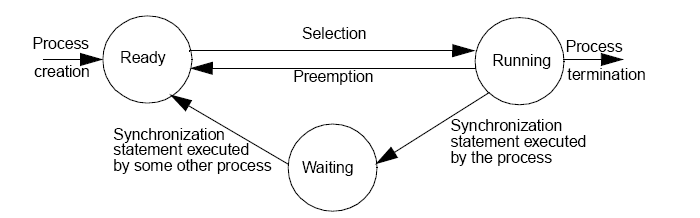
\includegraphics[scale=0.8]{img/preemtive.png}
\caption{Modello preemtive}\label{fig:preemtive}
\end{figure}
\subsection{I thread in C}
Tutti i sistemi UNIX sono multitasking con il sistema preemptive; tradizionalmente tutti i processi sono creati allo stesso modo tramite l'uso della primitiva \texttt{fork()}. La \emph{fork}produce una copia del processo chiamante; questa copia è esattamente identica all'origina tranne per il valore restituito dalla \texttt{fork} che per il processo figlio vale \emph{0} mentre nel padre il valore restituito è il \emph{pid} del figlio. Un piccolo esempio:
\begin{lstlisting}[language=C,float=htb,captionpos=b,caption={Esempio di uso della fork},label=lst:fork]
/*do parent stuff*/
ppid = fork ();
if (ppid < 0) {
	fork_error_function ();
} else if (ppid == 0) {
	child_function ();
} else {
	parent_function ();
}
\end{lstlisting}
La fork restituisce due copie completamente indipendenti dello stesso processo, questa indipendenza permette la protezione della memoria e la stabilità ma causa dei problemi quando si vuole che diversi processi lavorino sullo stesso problema; infatti sarebbe necessario usare \emph{pipes} oppure \emph{SysV IPC}. Inoltre il costo di switching tra processi multipli è molto alto, la sincronizzazione è lenta ed esistono dei limiti sul numero di processi che possono essere schedulati efficacemente.\\
Per questo sono stati introdotti i threads che invece possono essere schedulati all'interno del processo e risolvono molti problemi del lavoro multi processo.
L'API più popolare per creare una applicazione multithread in ambiente UNIX è la \emph{pthread} (\emph{POSIX thread}).\\
Le operazioni che si possono eseguire con quest'API sono la creazione, la distruzione, la sincronizzazione (\emph{join}), lo scheduling, il controllo dei dati e l'interazione con il processo principale. I threads dello stesso processo condividono le istruzioni di processo, gran parte dei dati, i descrittori dei file aperti, i segnali e lo user e il group id. Mentre per ogni thread abbiamo un distinto \emph{ThreadID}, un certo numero di registri, uno stack pointer ed una certa priorità come possiamo vedere \figurename~\ref{fig:threadstack}.
\begin{figure}[hbt]
\subfigure[]{
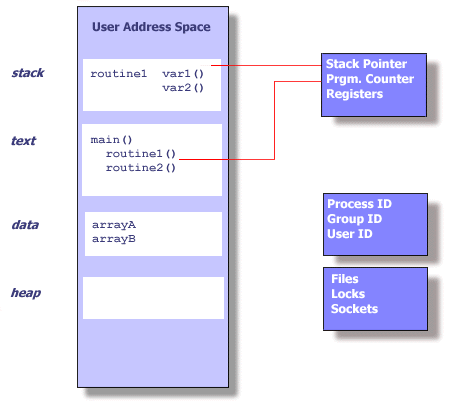
\includegraphics[width=7.5cm]{img/stack.png}
\label{fig:stack}
}
\subfigure[]{
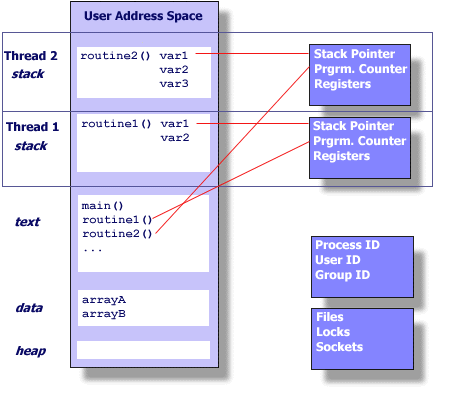
\includegraphics[width=7.5cm]{img/threadstack.png}
\label{fig:stackthread}
}
\caption{Memoria nel caso di processo (a) e di thread (b)}\label{fig:threadstack}
\end{figure}
Vediamo ora quali sono le funzioni della API \emph{pthread}
\paragraph{Thread creation}
La funzione per la creazione dei thread è:
\begin{lstlisting}[language=C,float=htb,captionpos=b,caption={Funzione di creazione dei thread},label=lst:creation]
int pthread_create (pthread_t *id, const pthread_attr_t *attr, void *(*routine)(void *), void *arg)
\end{lstlisting}
dove i valori sono:
\begin{description}
\item[id:] un valore che identifica il thread che viene restituito dalla funzione.
\item[attr]: un attributo che può essere utilizzato per impostare alcuni valori del thread. Se viene impostato a \emph{NULL} vengono impostati i valori di default.
\item[routine:] indica la funzione C che il thread eseguirà una volta creato.
\item[arg:] un singolo argomento che può essere passato a\texttt{routine}, deve essere passato come riferimento ad un puntatore di tipo \texttt{void}; in caso non vi siano valori si imposta a \emph{NULL}.
\end{description}
\paragraph{Thread termination}
Esistono diversi modi in cui un pthread può terminare:
\begin{itemize}
\item Il thread termina la sua routine.
\item Nel thread viene richiamata la \texttt{pthread\_exit}.
\item Il thread è cancellato da un altro thread tramite la chiamata della funzione \texttt{pthread\_cancel}.
\item L'intero processo termina quando viene chiamata una delle funzioni \texttt{exec} o \texttt{exit}.
\end{itemize}
Tramite la \texttt{pthread\_exit} è possibile specificare uno stato di terminazione che può essere restituito alla sincronizzazione del thread. Inoltre è molto importante ricordare che la \texttt{pthread\_exit} non chiude i file ed ogni file aperto all'interno del thread rimane aperto anche alla sua terminazione.
Se la funzione \emph{main} termina con una \texttt{pthread\_exit} prima che i threads siano conclusi i threads proseguono la loro esecuzione altrimenti terminano alla conclusione del \emph{main}.
Vediamo un esempio di creazione e terminazione dei thread in C nel Listato \ref{lst:thread}
\lstinputlisting[language=C,caption={Esempio di uso della API pthread},label=lst:thread]{listati/ThreadExample1.c}
\paragraph{Passaggio di argomenti}
Come abbiamo visto nella \emph{pthread\_create} è possibile impostare l'ultimo attributo con un attributo da passare alla routine che il thread eseguirà. Tale attributo deve essere convertito in un puntatore di tipo void. Tale passaggio presenta però alcuni tranelli, vediamo come nel Listato \ref{lst:wrongpass} come il passaggio per indirizzo crei un errore nell'esecuzione. Infatti, provando ad eseguire tale programma si rischia che più di un thread acceda contemporaneamente alla variabile \emph{t} e si rischiano quindi di ottenere dei valori sbagliati.
\begin{lstlisting}[language=C,caption={Errore nel passaggio di argomenti ad un thread},label=lst:wrongpass]
int rc, t;
for(t=0; t<NUM_THREADS; t++) {
	printf("Creating thread %d\n", t);
	rc = pthread_create(&threads[t], NULL, PrintHello, (void *) &t);
	...
}
\end{lstlisting}
Un possibile risultato di questo codice è quello seguente dove si può vedere che il thread numero 3 stampa il valore 4 anche se il thread numero 4 non è ancora stato creato (In realtà tutti i thread accedono alla variabile \emph{t} con un ritardo in quanto manca la stampa del thread numero 0).
\begin{verbatim}
Creazione del thread 0
Creazione del thread 1
1: Hello World!
Creazione del thread 2
2: Hello World!
Creazione del thread 3
3: Hello World!
4: Hello World!
Creazione del thread 4
\end{verbatim}
Per passare un argomento ad una routine è necessario controllare l'accesso ai dati da parte dei threads in modo che non vi siano possibili conflitti come nel caso del Listato \ref{lst:rightpass}. Nel quale viene passato ad ogni routine un puntatore ad un dato diverso.
\begin{lstlisting}[language=C,caption={Metodo corretto nel passaggio di argomenti ad un thread},label=lst:rightpass]
int *taskids[NUM_THREADS];
for(t=0; t<NUM_THREADS; t++) {
	taskids[t] = (int *) malloc(sizeof(int));
	*taskids[t] = t;
	printf("Creating thread %d\n", t);
	rc = pthread_create(&threads[t], NULL, PrintHello, (void *) taskids[t]);
	...
}
\end{lstlisting}
\paragraph{Joining threads}
L'operazione di \emph{join} è uno dei modi nel quale si può implementare la sincronizzazione tra thread.
\begin{lstlisting}[language=C]
int pthread_join(pthread_t thid,void **thread_return)
\end{lstlisting}
dove i diversi campi sono:
\begin{description}
\item[thid] è l'identificativo del thread su cui fare la join
\item[thread\_return] è il possibile valore di ritorno che si ottiene dall'invocazione della \texttt{pthread\_exit}
\end{description}
Il funzionamento della funzione di \emph{join} è specificato in \figurename\, \ref{fig:join}
\begin{figure}[htb]
\centering
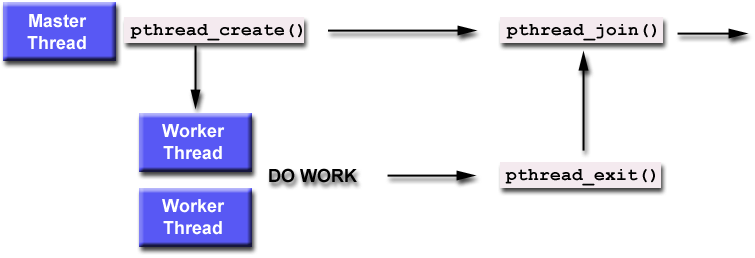
\includegraphics[scale=0.7]{img/join.png}
\caption{Funzionamento dell'operazione di join}\label{fig:join}
\end{figure}
\paragraph{I mutex}
Un \emph{mutex} funziona come un \emph{lock} proteggendo l'accesso a dei dati condivisi. Il concetto principale è che un solo thread alla volta può bloccare una variabile di tipo mutex, se più thread tenta di bloccare un mutex soltanto uno di questi effettuerà l'operazione con successo, inoltre i thread non possono bloccare un determinato mutex finché il thread che lo detiene non lo libera.\\
\uppercase{è} compito del programmatore assicurarsi che ogni thread che utilizza dei dati condivisi usi i mutex.\\
Una variabile di tipo mutex può essere dichiarata sfruttando la parola chiave \texttt{pthread\_mutex\_t}, per inizializzare tale variabile, invece, è possibile sfruttare due metodi:
\begin{itemize}
\item Il primo è l'inizializzazione statica come ad esempio
\begin{verbatim}
pthread_mutex_t mymutx = PTHREAD_MUTEX_INITIALIZER;
\end{verbatim}
\item Il secondo metodo è l'inizializzazione dinamica richiamando la routine
\begin{verbatim}
pthread_mutex_init
\end{verbatim}
In questo caso è possibile impostare alcuni parametri dell'oggetto mutex tramite le primitive \texttt{pthread\_mutexattr\_init} e \texttt{pthread\_mutexattr\_destroy} che rispettivamente creano e distruggono gli attributi  di un mutex
\end{itemize}
In entrambi i casi di inizializzazione l'oggetto mutex è inizializzato \emph{unlocked}. Infine, la routine \texttt{pthread\_mutex\_destroy} permette di rilasciare un mutex di cui non si ha più bisogno.\\
Esistono tre primitive per la gestione dei mutex, queste sono:
\begin{itemize}
\item \texttt{pthread\_mutex\_lock:} che si usa per acquisire un lock su di una variabile, nel caso in cui tale lock sia detenuto da un altro thread il thread che ha richiesto il lock si blocca finché il blocco non viene rilasciato.
\item \texttt{pthread\_mutex\_trylock} molto simile alla routine precedente solo che nel caso in cui il blocco sia detenuto da un altro thread allora la routine restituisce un codice di errore che indica \emph{"busy"}; è molto utile nel caso si vogliano prevenire condizioni di deadlock.
\item \texttt{pthread\_mutex\_unlock:} questa routine permette di rilasciare il lock in possesso del thread ma restituisce un errore nel caso in cui si voglia rilasciare un lock su di una variabile già sbloccata o bloccata da un altro thread.
\end{itemize}
\lstinputlisting[language=C,caption={Esempio di uso delle variabili mutex},label=lst:mutex]{listati/ThreadExample2.c}
\paragraph{Condition variables}
Mentre i mutex implementano la sincronizzazione tramite il controllo degli accessi sui dati le \emph{condition variables} permettono ai thread di sincronizzarsi in base ad un determinato valore di un dato. Senza quest'aspetto dei thread bisognerebbe implementare un polling per verificare quando una particolare condizione viene riscontrata. Le \emph{condition variables} sono un modo per ottenere lo stesso risultato senza il polling, e possono essere utilizzate anche insieme ai mutex.
L'utilizzo principale sono tutti quei problemi della categoria\textbf{produttore-consumatore}.\\
Come per i mutex le condition variabile sono dichiarate utilizzando la parola chiave \texttt{pthread\_cond\_t}; per l'inizializzazione esistono due metodi:
\begin{itemize}
\item Statico
\begin{verbatim}
pthread_cond_t myconvar = PTHREAD_COND_INITIALIZER
\end{verbatim}
\item Dinamico tramite la funzione \texttt{pthread\_cond\_init} che permette di settare anche gli attributi della variabile tramite le due primitive
\begin{verbatim}
pthread_condattr_init
pthread_condattr_destroy
\end{verbatim}
Che permettono rispettivamente di inizializzare e distruggere gli attributi della variabile
\end{itemize}
Infine tramite la primitiva \texttt{pthread\_cond\_destroy} è possibile liberare una variabile condizionale che non è più necessaria.\\
Per la gestione di questo tipo di variabile esistono diverse primitive:
\begin{itemize}
\item \texttt{pthread\_cond\_wait} è una routine che il thread finché una determinata condizione non si verifica, se chiamata quando vi è un lock attivo la routine sblocca il mutex e lo blocca nuovamente quando il thread si sveglia.
\item \texttt{pthread\_cond\_signal} questa routine risveglia gli altri thread in attesa di una \emph{condition variables}
\item \texttt{pthread\_cond\_brodcast} può essere utilizzata al posto della routine precedente se ci sono più thread bloccati in uno stato di \emph{"wait"}.
\end{itemize}
\subsection{Concorrenza in Java}
Come per il C anche il Java fornisce il supporto alla concorrenza a livello di linguaggio, esso mette a disposizione delle classi per istanziare ed eseguire nuovi thread più i metodi di sincronizzazione e le variabili di condizione.
Il modo più semplice per creare un thread è quello di utilizzare la classe \texttt{java.lang.Thread} in questo caso è sempre necessario implementare un metodo \texttt{run()}.
\begin{lstlisting}[language=Java,caption={Uso della classe Thread in Java},label=lst:jthread]
public class MyThread extends Thread {
	private String message;
	public MyThread(String m) {message = m;}
	public void run() {
		for(int r=0; r<20; r++)
			System.out.println(message);
	}
}

public class ProvaThread {
	public static void main(String[] args) {
		MyThread t1,t2;
		t1=new MyThread("primo thread");
		t2=new MyThread("secondo thread");
		t1.start();
		t2.start();
	}
}
\end{lstlisting}
Come vediamo la nostra classe che implementa un thread estende l'oggetto \emph{Thread}, in questa classe viene fatto l'override del metodo \texttt{run()} il quale non è altro che la routine che viene eseguita dal thread. Per far partire il thread è necessario richiamare il metodo \texttt{start()} dopo aver creato un nuovo oggetto.\\
Un'altra possibile soluzione è l'utilizzo dell'interfaccia \texttt{Runnable} la quale specifica soltanto che deve esistere un metodo \texttt{run()} che deve essere implementato. La classe \texttt{Thread} implementa anch'essa l'interfaccia \texttt{Runnable}.
Come vediamo nel Listato\,\ref{lst:runnable} a differenza del caso precedente oltre all'oggetto \emph{MyThread} deve anche essere creato un oggetto \emph{Thread} corrispondente, al quale viene poi passato l'oggetto MyThread, ed infine il metodo \texttt{start()}viene invocato sull'oggetto Thread.
\lstinputlisting[language=Java,caption={Utilizzo dell'interfaccia Runnable},label=lst:runnable]{listati/MyThread.java}
L'esecuzione dei thread non segue un ordine predefinito ma lo stesso codice può produrre risultati diversi su diversi computer o addirittura sullo stesso. Questo caratteristica è chiamata \emph{non-determinismo} ed è un punto focale nella concorrenza.\\
Java di per se implementa il modello \emph{preemtive} e nel caso sia disponibile un meccanismo di \emph{time-slicing} allora java esegue i thread con la stessa priorità tramite una meccanismo di \emph{round-robin}.\\
Per definire quando un sistema multithread è corretto si devono rispettare due proprietà:
\begin{itemize}
\item\emph{Sicurezza:} Un sistema si dice sicuro quando gli eventi malevoli non accadono.
\item\emph{Longevità:} Un sistema è longevo quando le cose buone possono accadere.
\end{itemize}
I possibili guasti che rientrano nella categoria "Sicurezza" sono quei guasti che avvengono a livello di esecuzione come i conflitti \emph{read/write} e \emph{write/write}. I meccanismi che invece riguardano la "Longevità" sono quei meccanismi che bloccano l'esecuzione del programma come:
\begin{itemize}
\item Lock
\item Waiting
\item CPU contention
\end{itemize}
Solitamente, purtroppo, le cose più semplici che si possono fare per aumentare la longevità ne riducono però la sicurezza e vice versa.\\
Vediamo ora quali sono i meccanismi che Java mette a disposizione per supportare la concorrenza.
\paragraph{Exclusion}
In un sistema sicuro ogni oggetto protegge se stesso da possibili violazioni della sua integrità. le tecniche di esclusione preservano l'invariante di un oggetto. Tre sono le tecniche principali per permettere l'\emph{esclusione}:
\begin{itemize}
\item Immutabilità
\item Esclusione dinamica (Locking)
\item Esclusione strutturale
\end{itemize}
Per quanto riguarda l'\textbf{immutabilità} si ottiene creando le classi in modo che gli oggetti proteggano se stessi come nel Listato\,\ref{lst:immutabile}
\begin{lstlisting}[language=Java,caption={Esempio di oggetto immutabile},label=lst:immutabile]
class ImmutableAdder {
	private final int offset;
	public Immutableadder (int a) {
		offset = a;
	}
	public int addOffset (int b) {
		return offset + b;
	}
}
\end{lstlisting}
I vantaggi di questa tecnica sono il fatto che non richiede sincronizzazione ed è molto utile per condividere degli oggetti tra i threads, ma sfortunatamente ha dei limiti di applicabilità.\\
Per parlare di sincronizzazione introduciamo prima l'esempio del Listato\,\ref{lst:sincro}
\begin{lstlisting}[language=Java,caption={Esempio sincronizzazione},label=lst:sincro]
public class RGBColor {
	private int r;
	private int g;
	private int b;
	
	public void setColor (int r, int g, int b)
		checkRGBVals(r, g, b);
		this.r = r;
		this.g = g;
		this.b = b;
	}
}
\end{lstlisting}
Ora immaginiamo che due thread chiamati \emph{red} e \emph{blue} vogliano impostare contemporaneamente il loro colore sullo stesso oggetto di tipo \texttt{RGBColor} a questo punto potrebbero verificarsi dei problemi in quanto i due thread tentano di scrivere lo stesso dato violando così la sua integrità.\\
Per risolvere questo problema java tramite il locking serializza l'esecuzione del codice dichiarato \emph{synchronized}. Ogni istanza di un oggetto possiede tali meccanismi di lock in quanto derivati dalla classe \texttt{Object}, l'unica eccezione si ha con l'utilizzo di array, infatti, bloccare un array non blocca gli elementi di tale array.\\
Esistono due modi per bloccare una parte di codice, si può dichiarare \emph{synchronized} un intero metodo o un singolo blocco di codice, in caso di singolo blocco la funzione \texttt{synchronized} richiede l'oggetto sul quale effettuare il lock (Listato\,\ref{lst:syncobj} e Listato\,\ref{lst:syncmeto}).\\
\pagebreak
\begin{lstlisting}[language=Java,caption={Sincronizzazione di una parte di codice},label=lst:syncobj]
synchronized (object) {
	//Lock is held
	...
}
//Lock is released
\end{lstlisting}
\begin{lstlisting}[language=Java,caption={Sincronizzazione di un metodo},label=lst:syncmeto]
synchronized void f() {
	//Lock is held
	/* Body */
}
//Lock is released
\end{lstlisting}
I lock vengono automaticamente acquisiti all'ingresso del blocco o del metodo dichiarato \texttt{synchronized} e rilasciato all'uscita da esso.\\
Alcune regole chiave per l'uso della sincronizzazione sono:
\begin{itemize}
\item Sempre quando si effettua un aggiornamento a dei campi di un oggetto.
\begin{lstlisting}[language=Java]
synchronized (point) {
	point.x = 5; point.y = 7;
}
\end{lstlisting}
\item Tutte le volte che si accede a dei dati che potrebbero essere aggiornati.
\begin{lstlisting}[language=Java]
synchronized (point) {
	if (point.x > 0) {...}
}
\end{lstlisting}
\item Si può fare a meno di sincronizzare parti di metodo stateless
\begin{lstlisting}[language=Java]
public void f() {
	synchronized (this) {
		state = ...;
	}
	operations();
}
\end{lstlisting}
\item \textbf{Mai} sincronizzare parti di codice che contengono invocazioni ad altri oggetti
\begin{lstlisting}[language=Java]
public void f() {
	synchronized (this) {
		...
	}
	h.foo();
}
\end{lstlisting}
\end{itemize}
La strategia più sicura (ma non la più efficace) per realizzare un'applicazione OO concorrente è quella di utilizzare oggetti completamente sincronizzati, anche detti oggetti \emph{atomici}, nei quali tutti i metodi sono sincronizzati, non esistono campi pubblici o altri tipi di violazione nell'incapsulamento, tutti i metodi sono finiti e hanno modo di rilasciare il lock, tutti i campi sono inizializzati ad un valore consistente nel costruttore, ed infine lo stato dell'oggetto è consistente sia all'inizio che alla fine di ogni metodo anche in presenza di eccezioni.\\
Uno dei problemi principali della programmazione concorrente è il \emph{deadlock}, tale problema si verifica quando due o più oggetti sono acceduti da due o più threads e tali thread detengono un lock mentre tentano di acquisire un lock detenuto da un altro thread.\\
L'assegnamento di un valore ad una variabile è un'operazione atomica (a parte per i \emph{long} e i \emph{double}), questo significa che generalmente non è necessario sincronizzare l'accesso ad una variabile. Tuttavia i thread solitamente memorizzano il valori delle variabile in memoria locale, questo significa che se un thread cambia il valore di una variabile un altro thread non vede il cambiamento. Per evitare questo meccanismo bisogna sincronizzare la variabile oppure dichiararla di tipo \texttt{volatile} che significa che ogni volta che una variabile è usata deve prima essere letta dalla memoria principale.\\
Il confinamento implementa l'incapsulamento garantendo che al massimo un'attività alla volta acceda agli oggetti. Questo meccanismo permette l'accesso ad un solo thread alla volta senza utilizzare i locking dinamici.
Il punto principale è quello avere un punto di uscita dal thread. Esistono quattro categorie per verificare che un riferimento \emph{r} ad un oggetto \emph{x} può uscire da un metodo \emph{m}:
\begin{itemize}
\item \emph{m} passa \emph{r} come argomento di un'invocazione ad un metodo o ad un costruttore di un oggetto
\item \emph{m} passa \emph{r} come valore di ritorno di un metodo.
\item \emph{m} registra \emph{r} in un campo accessibile da altre attività
\item \emph{m} rilascia un riferimento che però permette l'accesso ad \emph{r}
\end{itemize}
Per quanto riguarda le collezioni, il framework \texttt{java.util.Collection}  basata su uno schema \emph{Adapter} permette la sincronizzazioni delle classi collection, infatti, ad eccezione di \texttt{Vector} e \texttt{Hashtable} le classi base per le collezioni (come \texttt{java.utili.ArrayList}) sono non sincronizzate. Sono state così costruite una serie di classi sincronizzate attorno alle classi base come la \texttt{Collection.synchronizedList}.\\
Come abbiamo detto prima però la sincronizzazione non è molto efficiente infatti richiamare un metodo sincronizzato richiede un tempo quattro volte maggiore rispetto a metodi non sincronizzati; inoltre, esso riduce la concorrenza e diminuisce le performance, infine non vi è alcun modo di controllare il meccanismo dei lock.\\
Con java versione 5 sono stati introdotti nuovi meccanismi di sincronizzazione come la \emph{sincronizzazione condizionata.} Prendiamo come esempio un parcheggio con una certa capacità e dei metodi che permettono l'arrivo e la partenza di automobili come esemplificato nel Listato\,\ref{lst:monitor}.
\begin{lstlisting} [language=Java,caption={Esempio di controllore di un parcheggio},label=lst:monitor]
public class CarParkControl {
	protected int space;
	protected int capacity;
	
	public CarParckControl (int n) {
		capacity = space = n;
	}
	
	syncronized public void arrive() {
		...; --space; ...;
	}
	syncronized public void depart() {
		...; ++space; ...;
	}
}
\end{lstlisting}
Come per il C esistono però dei metodi che permettono una gestione più efficiente del controllore rispetto all'uso della syncronized; questi metodi sono:
\begin{itemize}
\item \texttt{public final void notify()}: che risveglia un singolo thread in attesa.
\item \texttt{public final void notifyAll()}: risveglia tutti i thread in attesa.
\item \texttt{public final void wait() throws InterruptedException}: pone il thread in attesa di un \emph{notify}. Quando un thread viene posto in uno stato di wait esso rilascia il lock acquisito e lo riacquista al suo risveglio.
\end{itemize}
\lstinputlisting[language=Java,caption={Esempio di variabili condizionali in Java},label=lst:jsincro]{listati/CarParkControl.java}
Si può ridurre l'overhead dovuto al contex-switching sostituendo la \texttt{notifyAll} con la \texttt{notify}. Tale meccanismo può essere usato per migliorare le performance quando si è certi che almeno un thread è in atteso per eseguire un lavoro.\\
Alla condizione di \emph{wait} è possibile associare un timer molto utile per migliorare la longevità del sistema in quanto tende a risolvere in modo automatico i deadlock.
\section{Comunicazione}\label{capitolo5}
La comunicazione tra processi è il cuore di tutti i sistemi distribuiti, infatti, non ha senso studiare i sistemi distribuiti senza esaminare come i processi su posti macchine diverse si scambiano le informazioni. La comunicazione nei sistemi distribuiti si basa sempre sullo scambio dei messaggi a basso livello come fornito dalla rete sottostante, anche se ciò rende la realizzazione del sistema distribuito molto complicata.\\
In questo capitolo analizzeremo prima di tutto le regole che i diversi processi devono rispettare per comunicare tra loro, queste regole sono conosciute anche come protocolli e solitamente vengono strutturati a livelli.\\
Analizzeremo in seguito tre modelli di comunicazione molto diffusi, le chiamate a procedure remote (RPC, \emph{remote procedure call}), i middleware orientati agli oggetti (MOM, \emph{message-oriented middleware}) e gli \emph{streaming} di dati. Ed infine analizzeremo il problema dell'invio di dati a destinatari multipli, ovvero, il \emph{multicast}.\\
\subsection{Il modello OSI}
A causa della mancanza di una memoria condivisa tutta la comunicazione nei sistemi distribuiti avviene mediante tramite l'invio e la ricezione di messaggi a basso livello. Quando un processo \emph{A} vuole comunicare con un processo $B$ prima di tutto costruisce un messaggio nel proprio spazio degli indirizzi e poi effettua una \emph{chiamata di sistema} che fa in modo che il SO si occupi dell'invio del messaggio attraverso la rete fino a raggiungere $B$. Anche se il principio è semplice esistono diversi ostacoli al completamente di questa operazione, prima di tutto $A$ e $B$ devono concordare sul significato dei bit inviati, esistono molti altri aspetti sui quali bisogna accordarsi, come il valore in volt usati per indicare un bit a 1, individuare l'ultimo bit del messaggio, bisogna inoltre capire se un messaggio è stato danneggiato o perso ecc.\\
Per poter trattare facilmente i numerosi aspetti di una comunicazione la \emph{international standards organization} (ISO) ha sviluppato un modello di riferimento che identifica i vari livelli di comunicazione coinvolti, gli assegna dei nomi standard e identifica le diverse funzionalità per ogni livello. Questo modello è chiamato \textbf{open system interconnection reference model} o più comunemente modello \textbf{ISO OSI} ed è illustrato in \figurename\,\ref{img:osi}
\begin{figure}[htb]
\centering
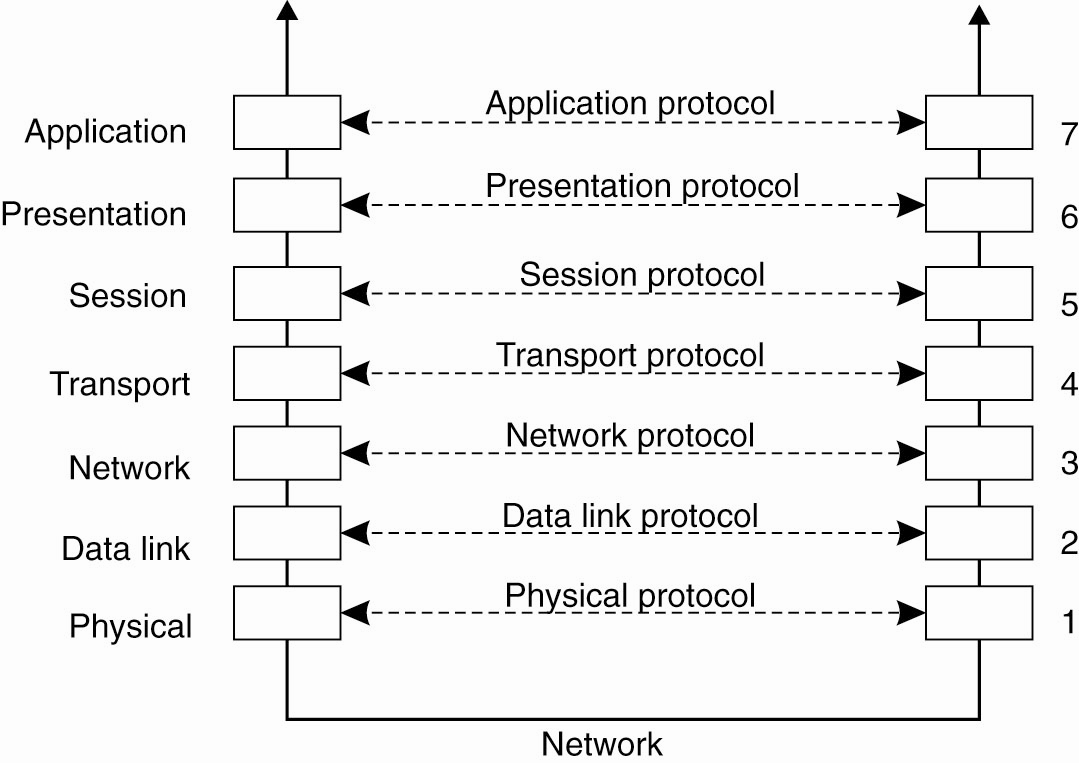
\includegraphics[scale=0.4]{img/osi.png}
\caption{Modello ISO OSI}\label{img:osi}
\end{figure}
Tuttavia è bene far presente che i protocolli sviluppati nel modello OSI non sono stati mai ampiamente utilizzati, tuttavia il modello sottostante si è rivelato particolarmente utile per comprendere le reti di computer.\\
Il modello OSI è progettato per consentire la comunicazione tra sistema aperti ovvero tra sistemi preparati per comunicare tramite regole standard che ne regolano il formato, i contenuti ed il significato di messaggi ricevuti ed inviati. Queste regole sono dette \textbf{protocolli} e devono essere concordate a priori per permettere la comunicazione tra gruppi di computer.\\
Esistono due grandi tipologie di protocolli, quelli \textbf{orientati alla connessione} nei quali mittente e destinatario stabiliscono esplicitamente una connessione prima di scambiarsi dei dati ed alla fine devono rilasciare tale connessione.
Con i protocolli \textbf{senza connessione} non è necessaria alcuna premessa, quando il messaggio è pronto il mittente invia il messaggio come nel caso di un invio di una lettera.\\
Nel modello OSI la comunicazione è suddivisa in sette livelli o \emph{layer}, ogni livello tratta uno specifico aspetto della comunicazione, in modo da suddividere il problema in parti gestibili ciascuna delle quali può essere trattata indipendentemente. Per realizzare questo meccanismo ogni livello fornisce un'interfaccia al livello superiore, la quale specifica un insieme di operazioni che il livello è pronto a fornire.\\
Quando un processo $A$ sulla macchina 1 vuole comunicare con un processo $B$ sulla macchina 2 costruisce un messaggio e lo passa al livello applicativo sulla sua macchina; tale livello potrebbe essere una procedura ad una libreria oppure implementato in qualche altro modo come ad esempio all'interno del sistema operativo. Il software a livello applicativo aggiunge un intestazione (\emph{header}) all'inizio del messaggio e passa tutto al livello di presentazione tramite l'interfaccia tra i livelli 6 e 7. A sua volta il livello di presentazione passa il messaggio al livello di sessione non prima di aver aggiunto il suo \emph{header} e così via. Alcuni livelli aggiungono oltre all'header anche un \emph{trailer} in chiusura al pacchetto come mostrato in \figurename\,\ref{img:header}.
\begin{figure}[htb]
\centering
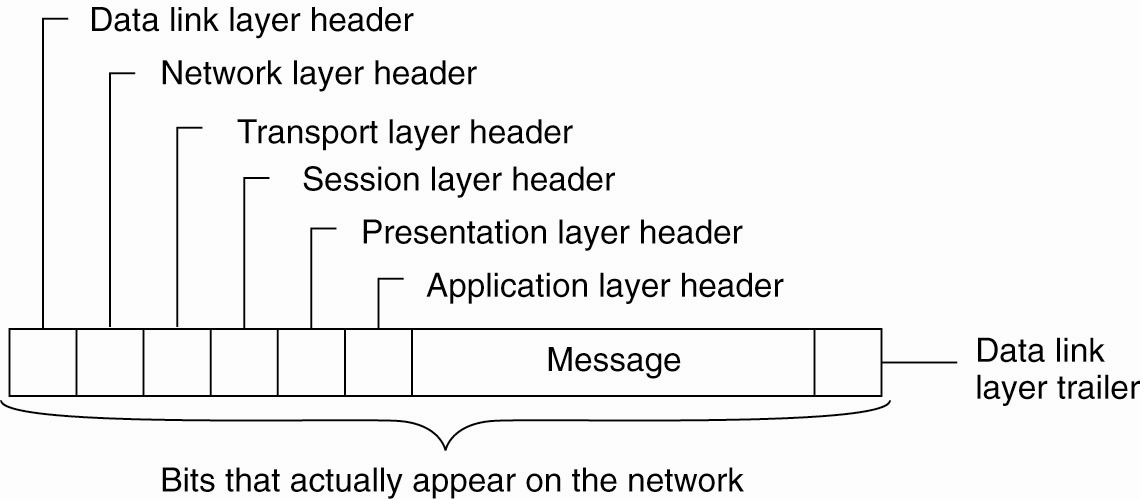
\includegraphics[scale=0.4]{img/header.png}
\caption{Elenco header e trailer di un messaggio che attraversa i vari layer}\label{img:header}
\end{figure}
Quando il messaggio raggiunge il fondo esso viene trasmesso dal livello fisico sul mezzo di trasmissione. Quando il messaggio raggiunge la macchina 2 viene passato verso l'alto e ogni livello stacca la sua intestazione e la esamina, infine il messaggio raggiunge il suo destinatario , ovvero il processo B il quale può rispondere utilizzando il percorso inverso.\\
Ogni livello ha il suo protocollo che può essere cambiato indipendentemente dagli altri ed è proprio questa indipendenza a rendere i protocolli a livelli interessanti.\\
L'insieme di protocolli usati in un particolare sistema è detto \textbf{suite di protocolli} o \textbf{stack di protocolli}.
\subsubsection{I layer}
Analizziamo ora i diversi layer che compongono il modello OSI, vedremo quali sono le loro funzionalità e dove possibile indicheremo quali protocolli sono attualmente utilizzati nell'ambito di internet.
Partiamo dai tre livelli più bassi della suite di protocolli, insieme questi tre livelli implementano le funzioni base di una rete di computer.\\
Il \emph{livello fisico} trasmette gli 0 e gli 1 sul canale fisico di comunicazione, elementi importanti per questo livello sono la quantità di volt che contraddistingue gli 0 e gli 1, il numero di bit al secondo, la possibilità di trasmettere in entrambe le direzioni, infine rivestono una notevole importanza la forma dei connettori (\emph{plug}) ed il numero di piedini (\emph{pin}). Il protocollo che identifica questo livello ha a che fare con la standardizzazione delle interfacce elettriche e meccaniche e di segnale; un esempio di questi standard è l'interfaccia RS-232-C per la comunicazione seriale.\\
Il livello \emph{data link} si occupa della rilevazione e della correzione degli errori di trasmissione. Per fare ciò il data link layer raggruppa i bit in unità chiamate \textbf{frame} e controlla che ogni frame sia ricevuto correttamente. Per eseguire questo compito il livello di collegamento dei dati applica un \emph{pattern} di bit all'inizio ed alla fine di ogni frame per delimitarli ed eseguire una \textbf{somma di controllo} (\emph{checksum}) sommando tramite algoritmi specifici i byte del frame ed inserisce tale somma nei campi all'inizio o alla fine del frame.
All'arrivo di un nuovo pacchetto il livello data link esegue la somma sui dati arrivati e la confronta con quella inviata insieme al pacchetto nel caso le due checksum coincidano il pacchetto è considerato corretto, in caso contrario il destinatario ne richiede la ritrasmissione grazie al numero di sequenza inserito nell'header del data link.\\
Il \emph{livello di rete} si occupa del \textbf{routing} dei pacchetti, ovvero, della scelta del percorso ottimale che permetta ad un pacchetto di andare da un mittente ad un destinatario.
Il problema si complica in quanto il percorso più breve non è sempre quello ottimo. Al momento il protocollo di rete più utilizzato è l'IP (\textbf{Internet Protocol}) senza connessione che è parte dei protocolli Internet. Un \textbf{pacchetto} IP può essere inviato senza alcun preparativo. Ogni pacchetto è instradato verso la sua destinazione indipendentemente da tutti gli altri.\\
Il \emph{livello di trasporto} costituisce l'ultima parte di quelli che possiamo definire \emph{stack del protocollo di rete di base} nel senso che implementa tutti i quei servizi non forniti dall'interfaccia del livello di rete ma necessari per l'implementazione di applicazioni di rete. In altre parole il livello di trasporto in un qualcosa di utilizzabile.\\
Uno dei compiti del livello di trasporto è quello di fornire una connessione affidabile anche se molte applicazioni gestiscono autonomamente la perdita di pacchetti.
Quando arriva un messaggio dal livello applicativo il livello di trasporto lo spezza in parti sufficientemente piccole per essere trasmesse ed assegna un numero di sequenza. Le informazioni nell'header del livello di trasporto riguardano il numero di pacchetti inviati, il numero di pacchetti ricevuti, quali devono essere ritrasmessi e così via.\\
Connessioni di trasporto affidabili possono essere costruite sopra servizi di rete orientati alla connessione o senza connessione. Nel primo caso i pacchetti arriveranno nella sequenza corretta, nel secondo caso non vi è alcun metodo per stabilire a priori l'ordine di arrivo dei pacchetti, ed è compito del software del livello di trasporto di riordinare i dati. Un aspetto importante del livello di trasporto è quello di fornire questo comportamento \emph{end-to-end}.\\
Il protocollo di trasporto di Internet è chiamato \textbf{TCP (transmission control protocol)}. La combinazione TCP/IP è oggi lo standard de facto per la comunicazione in rete. Oltre al TCP esiste anche un protocollo di trasporto senza connessione chiamato UDP (\emph{universal datagram protocol}) che è molto simile all'IP con alcune aggiunte minori.\\
Ulteriori protocolli sono proposti regolarmente, un esempio è il \textbf{real-time transport protocol (RTP)} il quale specifica il formato dei pacchetti per il trasferimento dei  dati in tempo reale ma non fornisce alcun meccanismo per garantire la loro consegna.\\
Sopra il livello di trasporto sono il modello OSI identifica altri tre livelli in realtà solo il livello applicativo è sempre usato. Per quanto riguarda i sistemi middleware nel il modello OSI nel l'approccio Internet sono soddisfacenti. Ad esempio il livello di sessione mette a disposizione funzionalità per il controllo del dialogo fornendo la possibilità di impostare \emph{checkpoint} che in caso di \emph{crash} permettano la ripresa della trasmissione senza ricominciare da capo. Tale meccanismo non è mai implementato nella suite di protocolli Internet. Tuttavia nel contesto di soluzioni middleware il concetto di sessione sono piuttosto cruciali.
Il compito del livello di prestazione è invece quello di dare un significato ai bit trasmessi. La maggior parte dei messaggi è composta da informazioni strutturate come nomi, indirizzi, quantità di denaro e così via. Nel \emph{livello di presentazione} è possibile definire dei \emph{record} contenenti campi come quelli precedentemente elencati in modo che il mittente possa comunicare al destinatario che il pacchetti contengono dei dati in un certo formato.\\
Il \emph{livello applicativo} era originariamente inteso per contenere semplici applicazioni di rete come l'e-mail o il trasferimento di file, ora è divenuto il contenitore di tutte le applicazioni. Ciò che manca in questo livello è una netta distinzione tra protocolli di una specifica applicazione e protocolli più generali.
\paragraph{Protocolli middleware}
Il middleware pur essendo posizionato in maniera logica nel livello applicativo contiene molti protocolli specifici che ne giustificano l'esistenza in un livello proprio. i protocolli per supportare una gran varietà di servizi middleware sono diversi, molti sono pensati per stabilire un autenticazione, non essendo legati ad una specifica applicazione questo tipo di protocolli può essere accorpato in un sistema middleware come servizio generale.
Un altro esempio di protocollo che rientra a far parte dei protocolli middleware è quello del \emph{commit distribuito} dove un operazione è portata a termine solo se è portata a termine in tutte le sue parti. Questa proprietà è detta \textbf{atomicità}ed è ampiamente utilizzata in tutti i tipi di transizioni.\\
Come abbiamo visto dai due esempi appena fatti i protocolli middleware supportano servizi di comunicazione di alto livello, ma oltre a questi esistono protocolli per supportare lo \emph{stream} di dati in tempo reale, oppure, protocolli più specifici del livello di trasporto ma che, dovendo tener conto dei requisiti delle applicazioni devono essere situati ad un livello più alto di quello di trasporto come ad esempio il caso di \emph{multicast} che devono garantire la scalabilità.\\
Il modello che si viene così a creare è quello di \figurename\,\ref{img:osimid} nel quale il livello di sessione e quello di presentazione vengono sostituiti da un unico livello middleware contenete quei protocolli indipendenti dalle applicazioni.
\begin{figure}
\centering
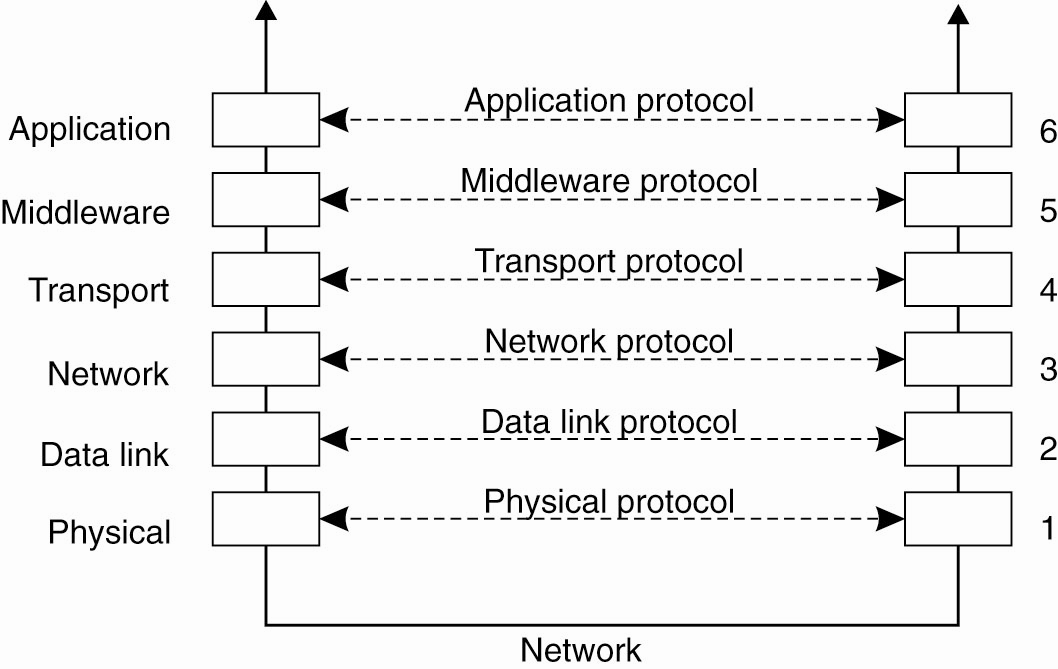
\includegraphics[scale=0.5]{img/osimid.png}
\caption{Modello OSI-Middleware}\label{img:osimid}
\end{figure}
\subsubsection{Tipi di comunicazione}
Esistono diverse alternative nella comunicazione che il middleware mette a disposizione delle applicazioni; partiamo dall'esempio mostrato in \figurename\,\ref{img:midcomuni}. In questo caso possiamo pensare che ogni \emph{host} esegua uno \emph{user agent} ovvero un processo che esegue le operazioni di comunicazione tra i vari sistemi.\\
\begin{figure}
\centering
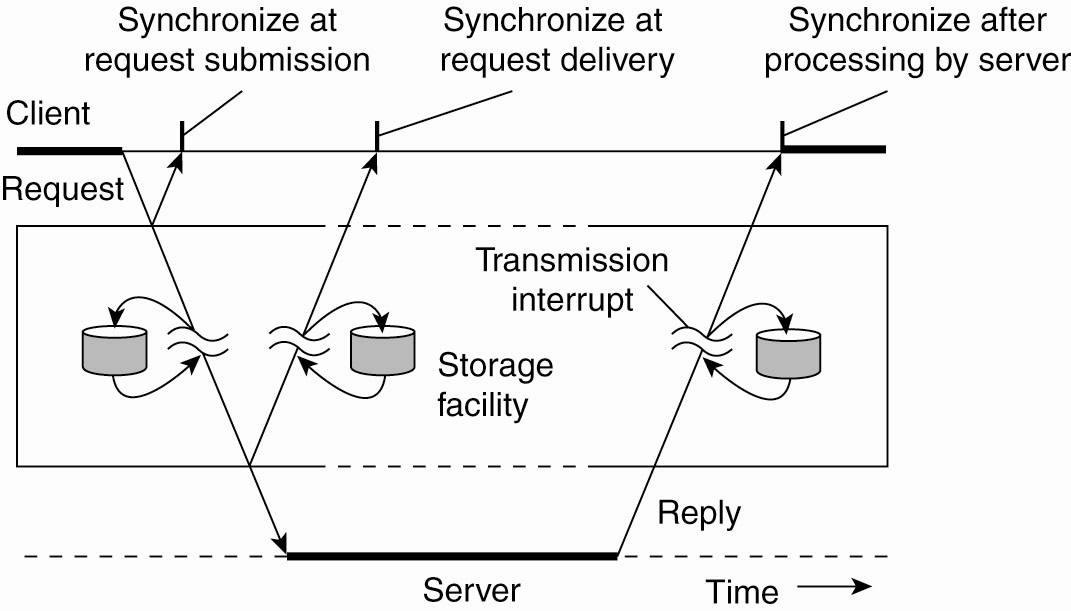
\includegraphics[scale=0.5]{img/midcomuni.png}
\caption{Esempio di tipi di comunicazione}\label{img:midcomuni}
\end{figure}
Prendiamo ora come esempio il caso di un invio di e-mail in questo caso i due \emph{user agent} saranno rispettivamente il sistema che invia e quello che riceve le e-mail. L'agente dal lato del mittente passa la mail al sistema per la consegna delle mail nella convinzione che tale sistema consegni la mail, l'agente dal lato del destinatario a sua volta si connette al sistema per sapere se è giunta qualche nuova mail in caso affermativo la mail viene trasferita dal sistema allo user agent del destinatario.\\
Questo tipo di meccanismo è detto \textbf{comunicazione persistente} in quanto il messaggio viene memorizzato dal middleware per tutto il tempo necessario affinché la consegna non vada a buon fine durante questo periodo non è necessario che i due elementi siano in esecuzione contemporaneamente. Nel caso di \textbf{comunicazione transiente} invece, il sistema memorizza i messaggi scambiati solo finché sia il mittente che il destinatario sono in esecuzione.\\
Oltre che persistente o transiente una comunicazione può essere asincrona o sincrona. Si parla di comunicazione \textbf{asincrona} quando il mittente continua la sua elaborazione subito dopo l'invio del messaggio. Nel caso di comunicazione \textbf{sincrona}, invece, il mittente è bloccato fino a quando la sua richiesta non viene accettata. Ciò può avvenire fino a quando il middleware non comunica la presa in consegna della richiesta, oppure quando la richiesta non viene consegnata al destinatario l'ultima possibilità è che il mittente resta bloccato fino alla fine dell'elaborazione da parte del destinatario e invio di una risposta all'elaborazione.\\
Esistono molti tipi in cui combinazione persistente, transiente, sincrona e asincrona possono essere combinati ma le più diffuse sono la persistenza e la sincronizzazione, la transiente con la sincronizzazione alla fine dell'elaborazione.\\
Dobbiamo distinguere, infine tra comunicazione discreta e a \emph{stream}.
\subsection{Chiamate a procedure remote}
Molti sistemi si basano sullo scambio di messaggi esplicito tra processi, questo scambio avviene tramite l'utilizzo delle procedure \texttt{send} e \texttt{recive} che però non nascondono del tutto la comunicazione. Una nuova tecnica fu introdotta nel 1984 quando si pensò di permettere ai programmi di richiamare procedure situate su altre macchine. Quando un processo sulla macchina $A$ richiama una procedura sulla macchina $B$ il processo chiamante viene sospeso e ha luogo l'elaborazione sulla macchina $B$. Le informazioni sono passate dal chiamante al chiamato tramite i parametri e ritornano indietro come risultato della procedura. Questo tipo di meccanismo è conosciuto come \textbf{chiamata a procedura remota } o \textbf{RPC} (\emph{remote procedure call}).\\
Sebbene l'idea di base risulti molto semplice i problemi relativi sono molti, primo fra tutti visto che chiamante e chiamata risiedono su due macchine diverse lo spazio degli indirizzi è completamente diverso, inoltre, il passaggio di parametri e dei risultati non è così semplice in quanto le macchine potrebbero avere rappresentazione dei dati differenti.
\subsubsection{Operazioni di base sulle RPC}
Iniziamo a vedere come funzionano realmente le RPC partendo dall'analisi di una chiamata a procedura locale per poi analizzare le chiamate remote.
\paragraph{Chiamate a procedura locali}
Per capire come lavorano le RPC è necessario capire comprendere come lavorano le chiamate a procedura convenzionali, ovvero su una singola macchina.
consideriamo una chiamate in C tipo:
\begin{center}
\texttt{count = read(fd, buf, nbytes)}
\end{center}
dove \emph{fd} è un intero che indica un file, \emph{buf} è un array di caratteri e \emph{nbytes} è il numero intero di byte da leggere ed immagazzinare in \emph{buf}.Se la chiamata è stata eseguita dal \emph{main} allora lo \emph{stack} della chiamata sarà quello mostrato in \figurename\,\ref{img:localstack}. Come vediamo nella figura (b) il chiamante inserisce (\emph{push}) i parametri nello stack in ordine inverso. Alla fine dell'esecuzione della procedura il valore di ritorno è posizionato in un registro vengono rimossi i parametri e viene restituito il controllo al chiamante.\\
\begin{figure}
\centering
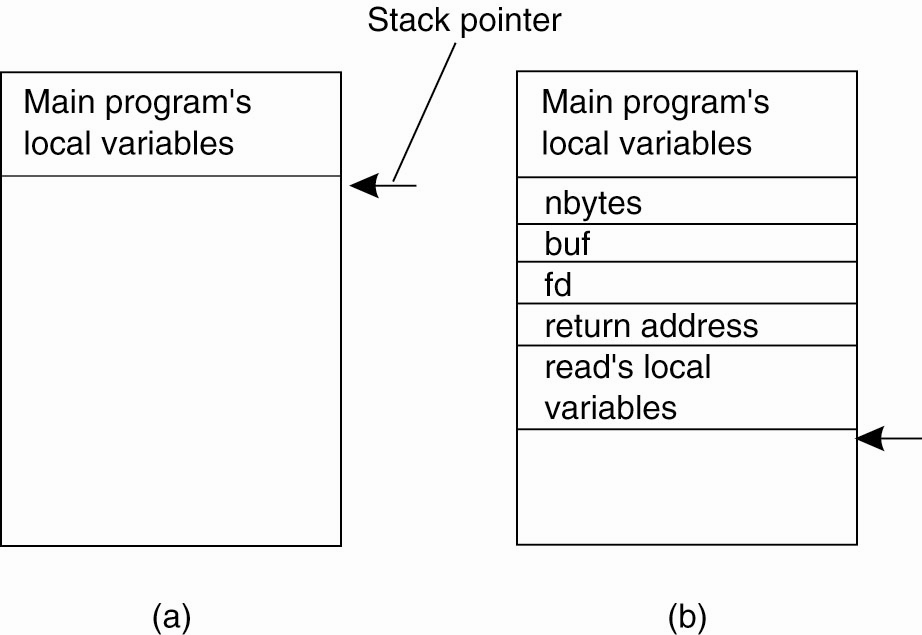
\includegraphics[scale=0.5]{img/localstack.png}
\caption{Stack prima e dopo la chiamata di una procedura}\label{img:localstack}
\end{figure}
Notiamo ora che in C i parametri possono essere passati per \textbf{valore} come \emph{fd} e \emph{nbytes} per i quali il valore viene copiato nello stack o per \textbf{referenza} come nel caso di \emph{buf} il quale è un puntatore ad un array di char; in questo caso nello stack della chiamata non vi è il valore dell'array ma semplicemente un indirizzo che indica dove l'array è situato. Nel caso in cui la procedura modifichi i valori contenuti nell'array tali cambiamenti saranno effettivi anche all'uscita dalla procedura.\\
Esiste un terzo meccanismo di passaggio dei parametri anche se non è usato in C ed è quello per \textbf{copia/ripristino}, questo passaggio consiste nel copiare il valore della variabile nello stack come nel caso di passaggio per valore, e quindi ricopiarla al termine della chiamata sovrascrivendo il valore originale. 
\paragraph{Client e server stub}
L'idea di base delle RPC è quella di rendere le chiamate a procedura remote il più simile possibile ad una chiamata locale. Vogliamo che le RPC siano trasparenti alla distribuzione. Per ottenere tale trasparenza quando il linker assembla il codice al posto di mettere la versione di sistema della procedura, nel nostro caso la \texttt{read}, esso la sostituisce con una versione chiamata \textbf{client stub}. Come quella originale anche questa versione viene richiamata usando la sequenza di \figurename\,\ref{img:localstack}, anche questa esegue una chiamata di sistema, ma a differenza di quella tradizionale questa chiamata impacchetta i dati in un messaggio e ne richiede l'invio al server tramite una \texttt{send}. Dopo l'invio il \emph{client stub} richiama la procedura \texttt{receive} e si blocca in attesa della risposta come mostrato in \figurename\,\ref{img:stub}.
\begin{figure}
\centering
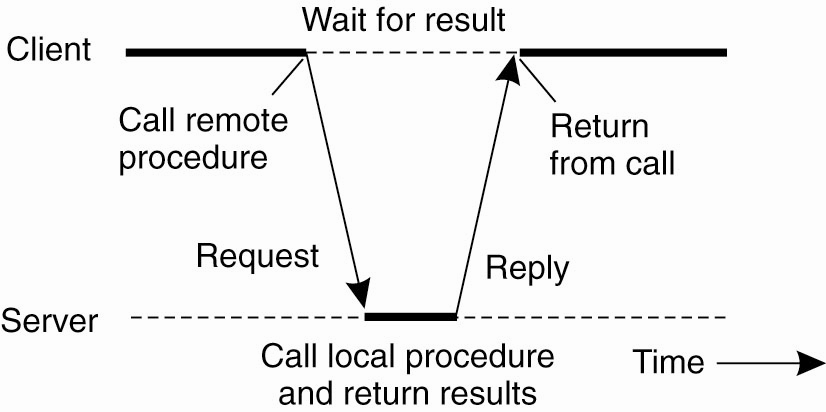
\includegraphics[scale=0.55]{img/stub.png}
\caption{Esempio di chiamata a procedura remota}\label{img:stub}
\end{figure}
Quando il messaggio raggiunge il server esso lo passa al \textbf{server sub}, l'equivalente lato server del \emph{client stub}, questo pezzo di codice trasforma la RPC in una chiamata a procedura locale. Il server esegue il proprio lavoro e restituisce il risultato al chiamante. Quando il \emph{server stub} riprende il controllo impacchetta il risultato in un messaggio e richiama la \texttt{send} per inviare la risposta al client e si rimette in attesa dell'arrivo di una nuova richiesta con la \texttt{receive}. Quando il messaggio di risposta arriva alla macchina client il sistema operativo lo indirizza al \emph{client stub} che lo spacchetta, copia i dati nel buffer e restituisce il controllo al processo client.\\
Quando il client riprende il controllo non ha idea di che cosa sia avvenuto e non ha idea se la chiamata è stata eseguita remotamente o in locale.
Ricapitolando una chiamata a procedura remota segue i seguenti passi:
\begin{enumerate}
\item la procedura client richiama il \emph{client stub} nel modo normale;
\item il \emph{client stub} costruisce un messaggio e richiama il sistema operativo locale;
\item il SO del client invia il messaggio al SO remoto;
\item il SO remoto passa il messaggio al \emph{server stub};
\item il \emph{server stub} spacchetta i parametri e richiama il server;
\item il server esegue il lavoro e restituisce il risultato allo \emph{stub};
\item il \emph{server stub} lo impacchetta in un messaggio e richiama il su SO;
\item il SO del server invia il messaggio al SO del client;
\item il SO del client passa il messaggio al \emph{client stub};
\item lo \emph{stub} spacchetta il risultato e lo restituisce al client.
\begin{figure}
\centering
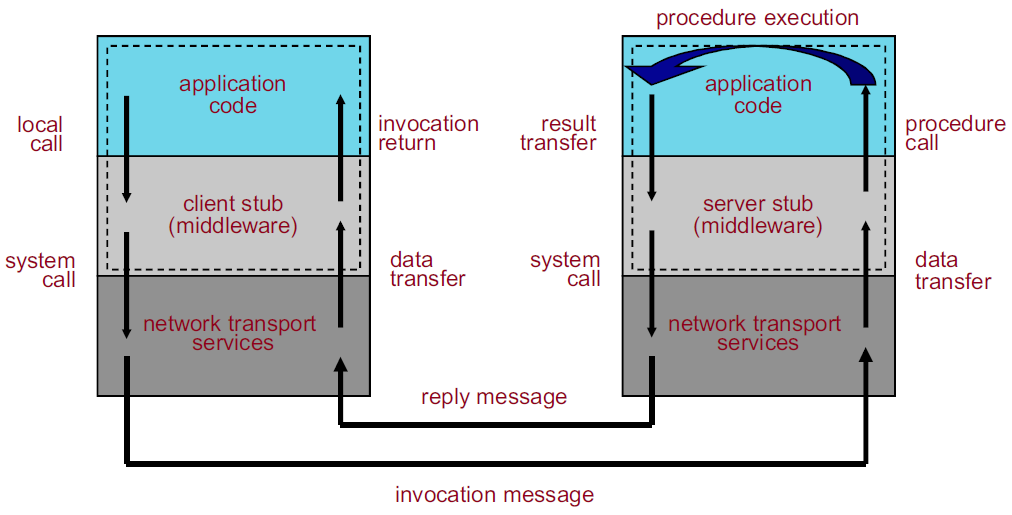
\includegraphics[scale=0.5]{img/execution.png}
\caption{Esecuzione di una chiamata a procedura a procedura remota}\label{img:executionrpc}
\end{figure}
\end{enumerate}
\subsubsection{Passaggio di parametri}
La funzione del client stub è quella di prendere i propri parametri di impacchettarli e di inviarli al server stub. Il problema è che questa operazione pur sembrando molto semplice in realtà non lo è.
\paragraph{Passaggio di parametri per valore}
\section{Naming}\label{capitolo6}
I nomi giocano un ruolo importante in tutti i sistemi di computer. Sono utilizzati per identificare, condividere e localizzare le diverse risorse. Un elemento importante del naming riguarda il fatto che un nome può essere risolto nell'entità a cui si riferisce, consentendo così ad un processo di accedere alla risorsa identificata da quel nome.\\
La differenza tra il \emph{naming} nei sistemi distribuiti e nei sistemi non distribuiti è data dal modo in cui questi sistemi sono implementati. In un sistema distribuito molte volte anche il meccanismo di \emph{naming} è distribuito per migliorarne efficienza e scalabilità.\\
Esistono diversi meccanismi di naming quelli che analizzeremo saranno quelli di tipo \emph{human-friendly} come quelli dei file system o del World Wild Web. L'altro meccanismo di naming che analizzeremo è quello relativo al naming di dispositivi mobili dove i nomi human-friendly non sono adatti ma sono utilizzati meccanismi in cui i nomi sono identificatori indipendenti dalla posizione oppure quelli che utilizzano hash table distribuite.
Infine analizzeremo quella tipologia di naming che esprimono le entità tramite varie caratteristiche attraverso l'utilizzo di attributi.
\subsection{Nomi,identificatori ed indirizzi}
Definiamo innanzi tutto che cos'è un nome. Un nome in un sistema distribuito è una stringa di bit o di caratteri utilizzata per riferirsi ad una entità. Un'entità può essere qualsiasi cosa, come host, stampanti, dischi o file; ma anche qualcosa che conosciamo meglio come processi, utenti, pagine web ecc.\\
Con tali entità noi possiamo interagire ma per fare ciò è necessario accedervi tramite un \textbf{punto d'accesso} (\emph{access point}) che non è altro che un tipo particolare di entità il cui nome è anche chiamato \textbf{indirizzo.}\\
Un entità può avere più di un punto d'accesso e può cambiarlo nel corso del tempo. Un indirizzo perciò è un tipo speciale di nome che si riferisce al punto di accesso di un'entità. Visto che il punto di accesso è strettamente legato all'entità sarebbe opportuno utilizzare l'indirizzo come nome regolare per riferirsi all'entità. Questa tecnica non è però applicabile in quanto solitamente l'indirizzo non è di facile comprensione e nemmeno flessibile. Prendiamo ad esempio il caso in cui un sistema distribuito sia riorganizzato e che un servizio prima disponibile su di una macchina sia ora riassegnato ad un server differente supponiamo inoltre che sulla vecchia macchina venga messo in funzione un nuovo servizio; a questo punto se abbiamo utilizzato un indirizzo per riferirci all'entità nel momento in cui il punto di accesso cambia o viene riassegnato abbiamo un riferimento non valido.\\
Questo esempio illustra come per un entità un nome differente dal suo indirizzo sia più facile e più flessibile. Tale tipologia di nome è detta \textbf{indipendente dalla posizione}.\\
Oltre agli indirizzi ci sono altri tipi di nomi che meritano una piccola analisi e sono quelli utilizzati per identificare univocamente un'entità. Questi nomi sono detti \textbf{identificatori} e rispettano le seguenti proprietà:
\begin{itemize}
\item un identificatore si riferisce al massimo ad una entità.
\item Ogni entità è referenziata da al massimo un identificatore.
\item Un identificatore si riferisce sempre alla stessa entità (non è mai riusato)
\end{itemize}
Usando gli identificatori diventa più facile riferirsi a un'entità in maniera non ambigua.\\
Indirizzi ed identificatori sono due importanti categorie di nomi impiegati per due scopi molto diversi. In numerosi sistemi tali nomi sono sono rappresentati in una forma leggibile dalla macchina ovvero sotto forma di bit. Al contrario i nomi \emph{\textbf{human-friendly}} sono rappresentati sotto forma di stringhe di caratteri in modo da essere usate dalle persone.\\
Il problema principale del naming risulta a questo punto essere quello di risolvere nomi e identificatori in indirizzi. In linea di principio un sistema di \emph{naming} mantiene un \textbf{collegamento nome-indirizzo} che nella sua forma più semplice è solo una tabella di coppie (\emph{nomi, indirizzo}). Tuttavia in sistemi distribuiti su di un ampia area geografica o di grandi dimensioni una tabella centralizzata non può funzionare.
Ciò che accade è che un nome viene scomposto in più parti e che la risoluzione del nome avviene in maniera ricorsiva
\subsection{Flat naming}
In precedenza abbiamo visto come gli identificatori sono adatti per rappresentare univocamente le entità tramite stringhe di bit molto semplici i quali per comodità vengono chiamati nomi non strutturati o semplici (\emph{flat}). Tali nomi non contengono alcuna informazione su come localizzare il punto d'accesso all'entità.
\subsubsection{Soluzioni semplici}
Analizziamo come primo meccanismo due semplici approcci per localizzare le entità in una rete locale.
\paragraph{Broadcasting e multicasting}
Consideriamo una rete che offre funzionalità di \emph{broadcasting} efficienti. Localizzare un'entità in tale ambiente è relativamente semplice, basta inviare un messaggio contenente l'identificatore dell'entità ad ogni macchina per verificare che tali macchine abbiano la risorsa. Solo le macchine che possono offrire un punto d'accesso per quella risorsa risponderanno al messaggio inviando l'indirizzo di quel punto d'accesso.\\
Questo principio è usato nel \textbf{protocollo di risoluzione degli indirizzi} (ARP \emph{address resolution protocol}) per trovare l'indirizzo a livello del collegamento dati \emph{(data-link)} di una macchina dato solo l'indirizzo IP.\\
In sostanza una macchina trasmette sulla rete locale un pacchetto richiedendo chi sia il proprietario di un determinato indirizzo IP. Quando un messaggio raggiunge una macchina controlla se ha l'indirizzo IP e in caso affermativo risponde al messaggio.\\
Tale meccanismo tuttavia diventa inefficiente man mano che la rete cresce, in quanto viene sprecata banda dalla grande quantità di messaggi inoltrati, inoltre molti host possono essere interrotti da richieste alle quali non possono dare una risposta. Una soluzione possibile è quella di passare al \emph{multicasting} nel quale solo un ristretto numero di host riceve la richiesta. Il \emph{multicasting} può essere usato per localizzare una risorsa nelle reti punto-a-punto, ad esempio, Internet supporta il \emph{multicasting} a livello di rete consentendo a diversi host di unirsi ad uno specifico gruppo di \emph{multicast}. Tali gruppi sono identificati da un \textbf{indirizzo multicast}. Quando un host invia un messaggio ad un indirizzo di multicast il livello di rete fornisce un meccanismo \emph{best-effort} per consegnare questo messaggio a tutti i membri del gruppo.\\
Un modo per utilizzare un indirizzo multicast potrebbe essere il caso di un azienda nel quale un PC,che chiameremo $A$, può essere connesso alla rete. Quando A viene connesso gli viene assegnato un indirizzo IP ed entra a far parte di un gruppo multicast. Nel caso un altro PC volesse contattare A dovrebbe prima di tutto localizzarlo e per fare ciò potrebbe inviare un messaggio "dov'è A?" a tutto il gruppo multicast, se A è connesso risponde con il suo indirizzo attuale.\\
Un altro modo per utilizzare un indirizzo di multicast è quello di associarlo ad un'entità replicata ed utilizzare il multicast per localizzare la replica più vicina.
\paragraph{Puntatori forwarding}
Un altro approccio molto diffuso per localizzare un'entità mobile è quella di utilizzare dei puntatori \emph{forwarding}. Il principio è abbastanza semplice, quando un'entità si sposta da A ad una nuova posizione B si lascia dietro un puntatore alla sua nuova posizione. Il vantaggio principale è la semplicità di realizzazione. Non appena viene trovata un'entità tramite \emph{naming service} tradizionale, un client può cercare l'indirizzo attuale seguendo la catena dei puntatori.\\
Esistono però anche una serie di inconvenienti; primo fra tutti se non vengono prese le opportune contromisure la catena di puntatori per un'entità molto mobile può diventare estremamente lunga e la sua localizzazione diventare molto dispendiosa. Inoltre ogni nodo intermedio della catena deve mantenere la sua parte di puntatori finché è necessario. Infine, il sistema è molto vulnerabile alla perdita di comunicazione, se viene perso uno dei puntatori la risorsa non è più raggiungibile. \uppercase{è} quindi fondamentale mantenere le catene di puntatori corte e i puntatori robusti.\\
Per capire il loro funzionamento prendiamo il caso dei puntatori \emph{forwarding} applicati agli oggetti remoti ai quali si accede tramite chiamate a procedure remote. Seguendo l'approccio delle \textbf{catene SSP} ogni puntatore è implementato come coppia (\emph{client stub, server stub}) come mostrato in \figurename\,\ref{img:forwarding}. Un server stub contiene un riferimento all'oggetto locale o un un riferimento ad un client stub remoto.\\
\begin{figure}
\centering
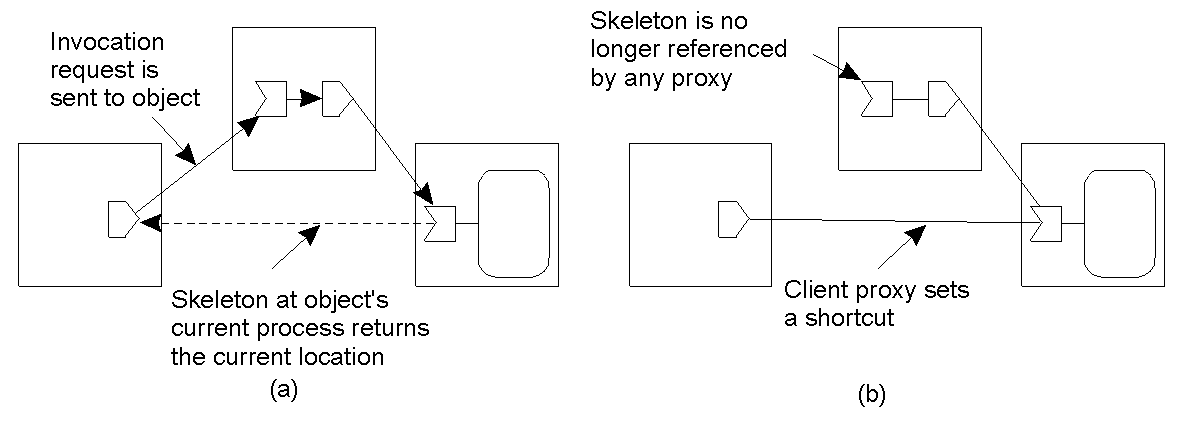
\includegraphics[scale=0.5]{img/forwarding.png}
\caption{Esempio di utilizzo di puntatori forwarding}\label{img:forwarding}
\end{figure}
Quando un oggetto si sposta dallo spazzio degli indirizzi di $A$ a quello di $B$ lascia su $A$ al suo posto un client stub che punta ad un server stub installato su $B$. Il punto focale è che la migrazione è completamente trasparente al client che contatta solo il client stub, gli è nascosto, invece, come e a quale posizione questo client inoltra le chiamate.\\
Per mantenere corta la catena una chiamata ad oggetto comporta l'identificazione del client che ha effettuato la chiamata tramite il suo indirizzo a livello di trasporto unito ad un numero generato localmente per identificare lo stub. Quando la chiamata arriva all'oggetto esso invia la risposta direttamente al client senza risalire la catena di puntatori, inoltre, insieme alla risposta viene inviata la posizione attuale dell'oggetto.\\
Si deve stabile un compromesso tra l'inviare una risposta direttamente al client stub oppure lungo la catena dei puntatori, nel primo caso la comunicazione è più veloce nel secondo invece è possibile aggiornare tutti i vari stub con la posizione aggiornata dell'oggetto.\\
Quando più nessun client fa riferimento ad un server stub, allora, quest'ultimo può essere rimosso. Tale operazione è strettamente collegata alla \emph{garbage collection} distribuita.
\subsubsection{Approcci home-based}
L'utilizzo del \emph{broadcasting} o di puntatori \emph{forwarding} comporta problemi di scalabilità. Un approccio diffuso per supportare entità mobili su reti di larga scala consiste nell'utilizzo della \textbf{home location} che tiene traccia della posizione attuale di un'entità. La home location di solito è il luogo dove è stata creata l'entità.\\
Il caso più comune nel quale si utilizzano gli approcci \emph{home-based} è quello dei Mobile IP dove ogni host ha un indirizzo IP fisso. Tutte le comunicazioni verso questo indirizzo viene inizialmente diretta verso \textbf{home agent} dell'host mobile. L'home agent è posizionato nella rete locale corrispondente all'indirizzo IP dell'host. Quando l'host mobile si sposta in un altra rete richiede un indirizzo temporaneo; questo \textbf{care-of-address} viene registrato dall'\emph{home agent}. Quando l'home agent riceve un pacchetto per l'host mobile cerca la posizione attuale dell'host, se l'host è nella rete locale allora il pacchetto semplicemente viene inoltrato, altrimenti, viene incanalato verso la posizione attuale dell'host e contemporaneamente il mittente del pacchetto viene informato sull'attuale posizione dell'host. Questo meccanismo è mostrato in \figurename\,\ref{img:homebase}.\\
\begin{figure}
\centering
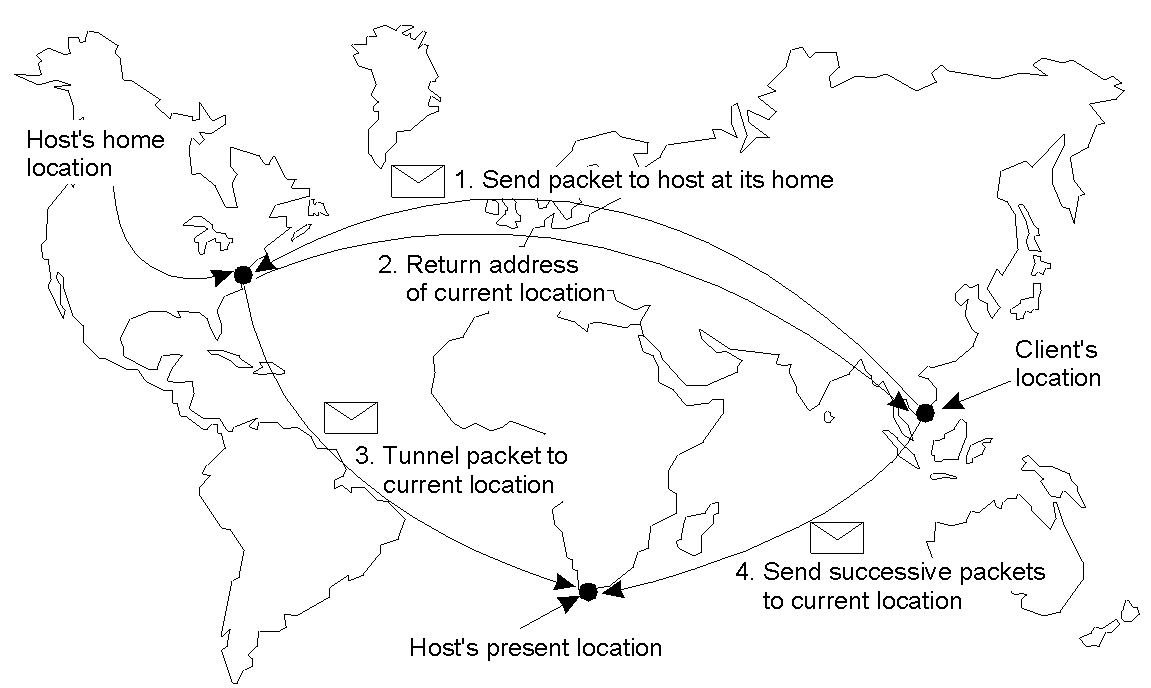
\includegraphics[scale=0.5]{img/homebase.png}
\caption{Il principio mobile IP}\label{img:homebase}
\end{figure}
Un inconveniente di questo meccanismo è che un host può essere molto lontano dalla sua home, il risultato è un aumento dei tempi di latenza. Inoltre, bisogna assicurare che la home location esista sempre altrimenti risulta impossibile contattare la risorsa.
\subsubsection{Hash table distribuite}
I recenti sviluppi hanno portato a possibili risoluzioni di un identficatore nell'indirizzo  di un elemento associato tramite l'utilizzo di \emph{hash table} distribuite. Nella concezione di base i meccanismi basati su SHT non tengono conto della vicinanza della rete, questo può causare problemi di prestazioni.
\paragraph{Meccanismo generale} 
Esistono diversi sistemi basati su DHT, il sistema \emph{Chord} è rappresentativo di molti di loro anche se esistono importanti differenze riguardo la complessità di gestione e i protocolli di ricerca.\\
Come abbiamo visto nel Capitolo \ref{capitolo2} Chord utilizza uno spazio degli identificatori a $m$ bit per assegnare degli identificatori casuali ai nodi e alle chiavi di una specifica entità. Il numero $m$ di bit è solitamente 128 o 160 a seconda della funzione di \emph{hash} utilizzata. Un'entità con chiave $k$ cade sotto la giurisdizione del nodo con il più piccolo identificatore $id \geq k$; questo nodo è chiamato il \emph{successore} di $k$ e indicato come $succ(k)$.\\
La questione principale in un sistema basato su DHT è quello di risolvere una chiave $k$ nell'indirizzo di $succ(k)$. Un approccio semplice ma che purtroppo non scala bene è di lasciare che ogni nodo $p$ tenga traccia del suo successore $succ(p+1)$ e del suo predecessore $pred(p)$. In questo caso quando un nodo $p$ riceve una richiesta la inoltra semplicemente ad uno dei suoi vicini a meno che la chiave che sta cercando non rispetti $pred(p) < k \leq p$, in questo caso il nodo $p$ deve restituire il suo indirizzo.\\
Diversamente da questo approccio lineare, ogni nodo Chord mantiene una \textbf{finger table} di al massimo $m$ elementi. Se $FT_p$ è la \emph{finger table} del nodo $p$ allora 
$$FT_p[i] = succ(p+2^{i-1})$$
Ovvero l'\emph{i-esimo} elemento punta al primo nodo successivo a $p$ di almeno $2^{i-1}$ posizioni. Questi riferimenti sono collegamenti a nodi realmente esistenti, dove la distanza del collegamento (\emph{short-cutted distance}) dal nodo $p$ cresce esponenzialmente man mano che aumenta l'indice della finger table.\\
Per individuare una chiave $k$ il nodo $p$ inoltra la richiesta al nodo $q$ con indice $j$ nella \emph{finger table} di $p$ dove
$$q = FT_p[j]\leq k < FT_p[j+1]$$
Per mostrare il funzionamento si rimanda alla \figurename\,\ref{img:chordexe} dove si mostrano i passaggi per la ricerca di una chiave $k = 7$ inoltrata al nodo 1.
Si può dimostrare che una ricerca richiede in genere $O(log(N))$ passi, dove $N$ sono il numero di nodi del sistema.\\
\begin{figure}
\centering
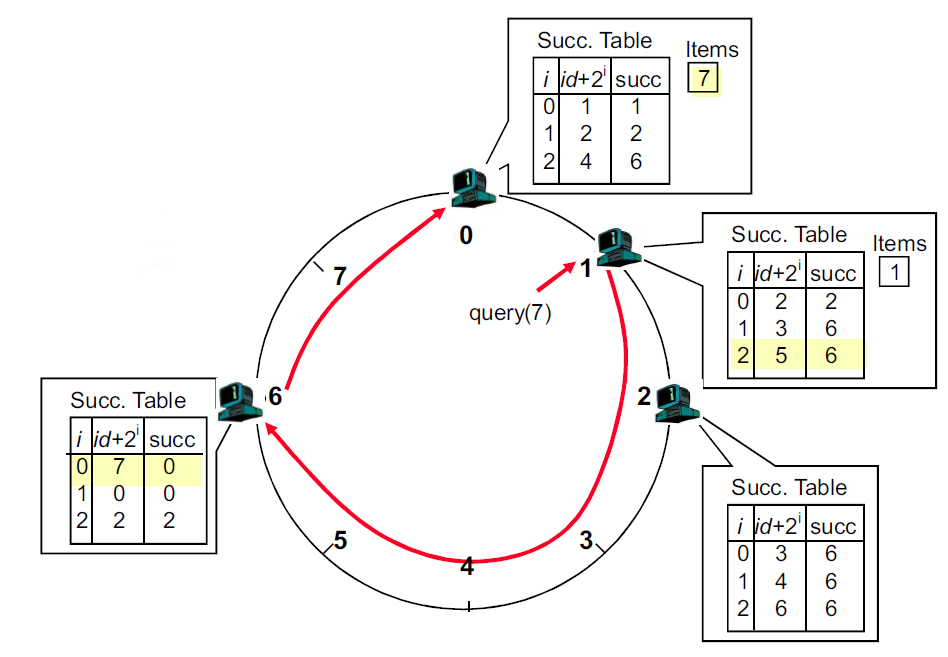
\includegraphics[scale=0.5]{img/chordexe.png}
\caption{Esempio di esecuzione di due ricerche}\label{img:chordexe}
\end{figure}
In un sistema distribuito ci si può aspettare che l'insieme dei nodi cambi continuamente, non solo i nodi entrano ed escono volontariamente ma possono anche subire dei guasti per poi tornare a funzionare successivamente.
Entrare in un sistema basato su DHT come \emph{Chord} è relativamente semplice. Supponiamo che un nodo $p$ voglia unirsi al sistema, esso contatta un nodo a caso del sistema e richiede la ricerca di $succ(p+1)$. Una volta identificato $p$ può unirsi all'anello. La complessità sta nel mantenere le \emph{finger table} aggiornate. La cosa più importante è che per ogni nodo $q$, $FT_q[1]$ (il successore) sia corretto. Per ottenere questo risultato ogni nodo $q$ esegue periodicamente una semplice procedura che contatta il $succ(q+1)$ e gli richiede di restituire $pred(succ(q+1))$. Se $q=pred(succ(q+1))$ allora $q$ è sicuro che le sue informazioni sono consistenti. Altrimenti nel sistema è entrato un nodo $p$ con $q<p\leq succ(q+1)$ per cui $q$ aggiornerà $FT_q[1]$ a $p$. A questo punto controllerà anche se $p$ ha memorizzato $q$ come suo predecessore. Se non fosse così allora è necessario un ulteriore aggiornamento di $FT_q[1]$.\\
Per aggiornare la finger table il nodo $q$ non deve far altro che contattare il successore di $k = q+2^{i-1}$ per ogni elemento $i$ della sua \emph{finger table}.
\paragraph{Sfruttare la vicinanza della rete}
Uno dei problemi principali del sistema Chord è che le richieste possono essere instradate in modo bizzarro, per minimizzare simili casi la progettazione di un sistema basato su DHT deve tener conto della rete sottostante.\\
Una prima soluzione potrebbe essere l'\textbf{assegnamento degli identificatori dei nodi basato sulla topologia}, in altre parole l'idea è quella di assegnare gli identificatori in modo tale che nodi vicini abbiano anche identificatori vicini. Questo meccanismo porta con sè però molte problematiche tra cui il \emph{mapping} di un anello logico su internet, che è un operazione non banale. Inoltre nel caso in cui una sottorete non diventi più raggiungibile si possono avere dei buchi consistenti negli identificatori che altrimenti avrebbero una distribuzione casuale.\\
Con l'\textbf{instradamento per vicinanza} (\emph{proximity routing}) i nodi mantengono una liste di alternative a cui inoltrare una richiesta. Per esempio preso un indice della finger table non si tiene conto solo del successore ma anche di $n$ successori nell'intervallo $[p+2^{i-1},p+2^i-1]$, ciò porta il sistema a poter scegliere a chi instradare una richiesta.\\
Infine nella \textbf{proximity neighbor selection} l'idea è quella di ottimizzare le tabelle di \emph{routing} in modo tale che il nodo più vicino sia selezionato come \emph{neighbor}. Non vi è molta differenza tra il \emph{proximity routing} e il \emph{proximity neighbor selection} in quanto nel proximity routing si scelgono $r$ alternative mentre nel proximity neighbor si scelgono gli $r$ vicini migliori.
\subsubsection{Approcci gerarchici}
L'approccio principale che presenteremo in questo paragrafo è basato sul servizio di localizzazione di \emph{Globe}. Si tratta di un servizio di localizzazione generico rappresentativo di molti sistemi di localizzazione gerarchici.\\
In uno schema gerarchico una rete è suddivisa in un insieme di \textbf{domini}. Esiste un solo dominio \emph{top-level} che comprende l'intera rete. Ogni dominio può essere suddiviso in molti sottodomini più piccoli, il dominio di livello più basso (\emph{lowest-level}) viene chiamato \textbf{dominio foglia} e corrisponde di solito ad una rete locale (LAN).\\
Ogni dominio $D$ ha un nodo directory associato $dir(D)$ che tiene traccia delle entità nel dominio. Questo meccanismo porta ad un albero di nodi directory con il nodo directory del dominio \emph{top-level} chiamato anche \textbf{nodo radice} il quale conosce tutte le entità. Tale organizzazione è mostrata in \figurename\,\ref{img:gerarchica}\\
\begin{figure}
\centering
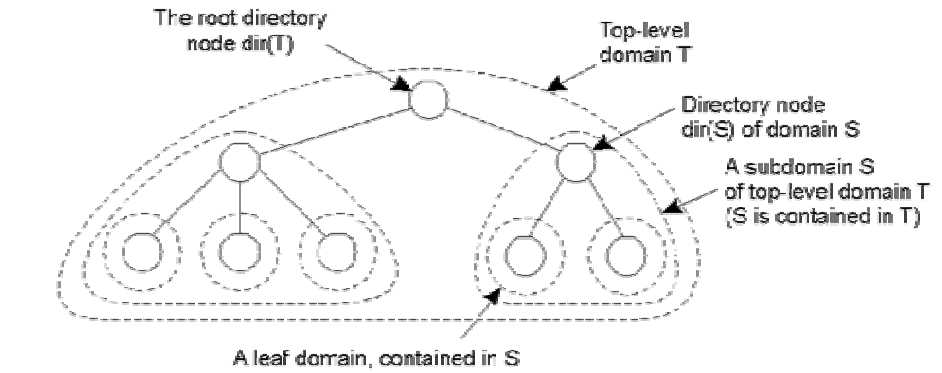
\includegraphics[scale=0.4]{img/gerarchico.png}
\caption{Esempio di organizzazione gerarchica}\label{img:gerarchica}
\end{figure}
Ogni entità attualmente posizionata in un dominio $D$ è rappresentata da un \textbf{location record} nel nodo directory $dir(D)$. Un \emph{location record} dell'entità $E$ nel nodo directory $N$ del dominio foglia $D$ contiene l'indirizzo attuale dell'entità in quel dominio. Mentre a livello superiore il \emph{location record} di $E$ conterrà un puntatore ad $N$.\\
Un'entità può avere molteplici indirizzi, ad esempio nel caso sia replicata. In tal caso il nodo directory del dominio più piccolo che contiene le due entità avrà due puntatori ai due sotto-domini per quell'entità coem mostrato in \figurename\,\ref{img:sottodomini}
\begin{figure}
\centering
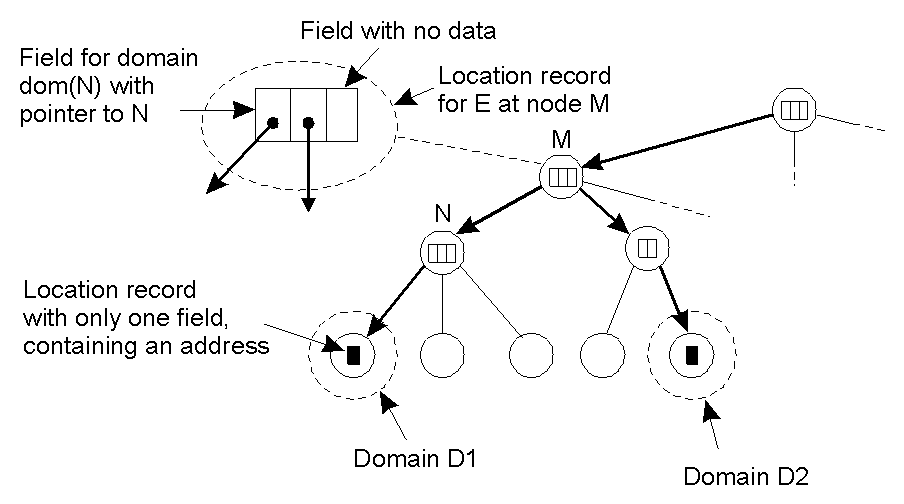
\includegraphics[scale=0.5]{img/sottodominio.png}
\caption{Esempio di memorizzazione delle informazioni nel caso di entità replicata}\label{img:sottodomini}
\end{figure}
Per quanto riguarda la ricerca in un sistema gerarchico avviene anch'essa in modo gerarchico ma con un approccio \emph{bottom-up}; se nel nodo directory non è presente un \emph{location record} per quell'entità allora il nodo inoltra la richiesta al padre, se anche il padre non ha un \emph{location record} per l'entità la richiesta risale l'albero fino a quando non trova un location record valido oppure non raggiunge la radice. Non appena una richiesta raggiunge un nodo directory $M$ contenente un \emph{location record} per l'entità $E$ sappiamo che $E$ si trova da qualche parte nel dominio $dom(M)$. A questo punto la richiesta viene inoltrata al nodo directory del sottodominio contente $E$ e così via procedendo fino a raggiungere una foglia, questo indirizzo può finalmente essere restituito al client che ha inoltrato la richiesta. Questo procedimento è illustrato in \figurename\,\ref{img:ricerca}
\begin{figure}
\centering
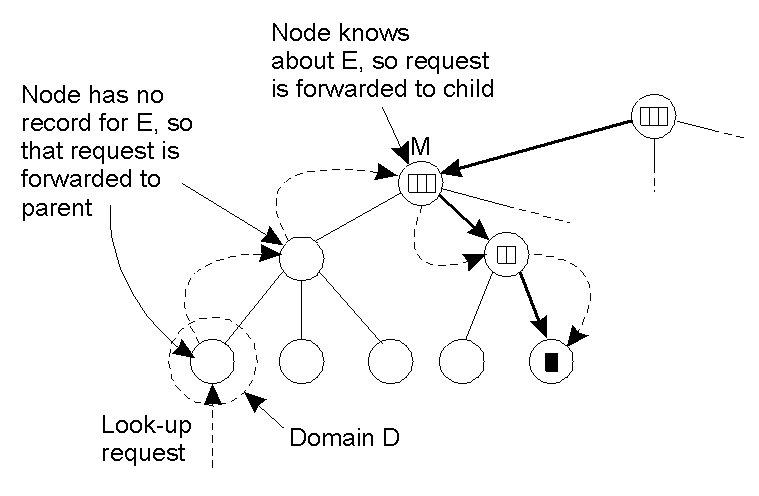
\includegraphics[scale=0.5]{img/ricerca.png}
\caption{Esempio di ricerca in un sistema gerarchico}\label{img:ricerca}
\end{figure}
Le operazioni di aggiornamento sfruttano lo stesso principio, l'inserimento avviene in un nodo foglia e il riferimento ad $E$ è propagato verso l'alto fino a quando in un nodo directory non si incontra già un riferimento ad $E$, a questo punto il nodo che ha già il \emph{location record} per e memorizza il nodo figlio dal quale è giunta la richiesta di inserimento, per installare la catena dei puntatori si possono applicare sia meccanismi \emph{top-down} (una volta raggiunto un nodo con un location record per $E$ si ridiscende l'albero impostando i diversi puntatori) oppure, un approccio \emph{bottom-up} (a mano a mano che la ricerca del location record di $E$ sale si instaurano i puntatori ad $E$). Nel secondo caso una risorsa diventa disponibile per un determinato dominio non appena la richiesta risale per il nodo directory di quel dominio.
\subsection{Naming strutturato}
I nomi semplici sono adatti per le macchine ma in generale non sono opportuni per gli uomini. Come alternativa i sistemi di \emph{naming} supportano i nomi strutturati composti da diversi nomi semplici e leggibili dall'uomo. Un esempio sono i nomi dei file, i nomi degli host di Internet e altri ancora.
\subsubsection{Name space}
I nomi sono solitamente organizzati nel cosiddetti \textbf{spazi dei nomi} o \emph{name space}. Uno spazio dei nomi può essere rappresentato come un grafo orientato nel quale esistono due tipi di nodi, i \textbf{nodi foglia} che rappresentano le diverse entità e può contenere soltanto informazioni come indirizzi, come nel caso di host oppure contenere direttamente tutto lo stato dell'entità come nel caso dei file system.\\
Esistono poi i \textbf{nodi directory} i quali hanno diversi archi in uscita ciascuno dei quali etichettato con un nome. Tuttavia questa è l'unica differenza in quanto in un grafo dei nomi ogni nodo è considerato come un'entità. Un nodo directory contiene una tabella in cui un arco in uscita è rappresentato da una coppia (\emph{etichetta dell'arco, identificatore del nodo}), tale tabella è chiamata \textbf{directory table}.\\
Un nodo che ha solo archi in uscita e nessun arco in entrata viene detto \textbf{nodo radice}. Ogni percorso in un grafo dei nomi può essere chiamato tramite una sequenza di etichette corrispondenti agli archi del percorso ad esempio
$$N:<label_1, label_2, \dots, label_n>$$
Tale percorso è detto \textbf{path name}. Se il primo nodo in un \emph{path name} è la radice del grafo è detto \textbf{path name assoluto} altrimenti è detto \textbf{path name relativo}.\\
Un \textbf{nome globale} è un nome che denota la stessa entità a prescindere da dove sia usato il nome all'interno del sistema. Diversamente un \textbf{nome locale} è un nome la cui interpretazione dipende da dove il nome viene usato. 
\subsubsection{Risoluzioni dei nomi}
Gli spazi dei nomi sono un meccanisomo adatto a memorizzare e recuperare informazioni sulle entità per mezzo dei nomi. Dato un path name dovrebbe essere possibile ricercare qualunque informazione memorizzata nel nodo cui il path name si riferisce. Il processo di ricerca in base a un nome è chiamato \textbf{risoluzione del nome} o \emph{name resolution}.\\
Per spiegare come funziona consideriamo il \emph{path name} precedente
$$N:<label_1, label_2, \dots, label_n>$$
La risoluzione di questo nodo comincia dal nodo $N$ del grafo dei nomi, viene poi ricercato il nodo con nome $label_1$ nella \emph{directory table}; ci si sposta poi in tale nodo e nella sua \emph{directory table} si ricerca il riferimento al nodo con nome $label_2$ e così via. Supponendo che tale path sia un percorso valido allora la risoluzione terminerà nell'ultimo nodo indicato da $label_n$ con la resttuzione del contenuto di quel nodo.
\paragraph{Meccanismo di chiusura}
La risoluzione di un nome può avvenire soltanto se sappiamo come e da dove iniziare, nel nostro esempio il nodo iniziale era specificato e sapevamo di aver accesso alla sua \emph{directory table}. Sapere come e da dove iniziare viene chiamato \textbf{meccanismo di chiusura}.\\
Un meccanismo di chiusura ha a che fare con la selezione del nodo iniziale in uno spazio dei nomi da cui deve iniziare la risoluzione. A volte però tali meccanismi sono di difficile comprensione in quanto molte volte impliciti e diversi gli uni dagli altri.\\
Per esempio nel file system di UNIX la risoluzione punta sul fatto che l'\emph{inode} della \emph{root directory} è il primo \emph{inode} nel disco logico.
\paragraph{Linking e mounting}
Strettamente correlato alla risoluzione dei nomi è l'uso di \textbf{alias}. Un alias è un altro nome per la stessa entità. Ad esempio una variabile d'ambiente come \texttt{\$HOME} è un esempio di alias. Ci sono fondamentalmente due modi per implementare un alias, il primo metodo è di consentire che molteplici path name assoluti si riferiscano allo stesso nodo  come mostrato in \figurename\,\ref{img:hardlink}. Questo approccio nei file system UNIX è chiamato \textbf{hard link}. 
\begin{figure}[htb]
\centering
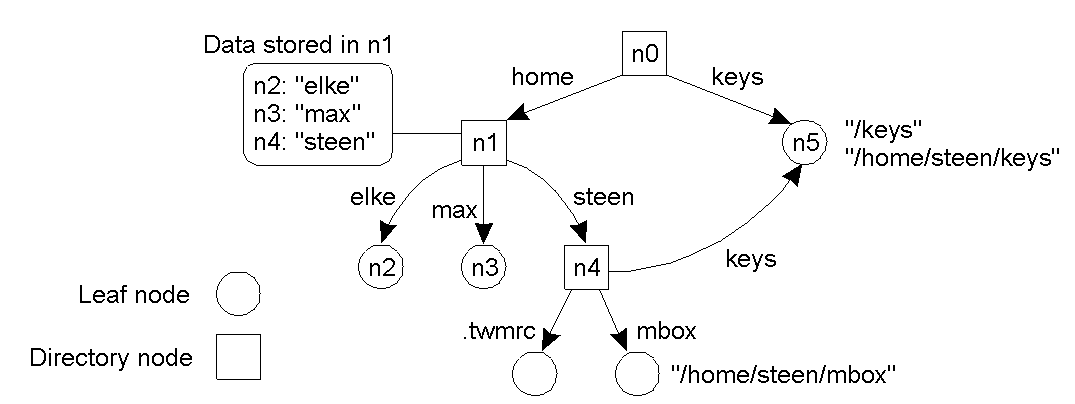
\includegraphics[scale=0.5]{img/hardlink.png}
\caption{Esempio di hard link}\label{img:hardlink}
\end{figure}
Il secondo metodo è quello di rappresentare un'entità tramite un nodo foglia il quale al posto di memorizzare l'indirizzo o lo stato dell'entità memorizza un path name assoluto come mostrato in \figurename\,\ref{img:symboliclink}. Questa volta, sempre riferendoci ai file system UNIX parliamo di \textbf{link simbolici}.
\begin{figure}[htb]
\centering
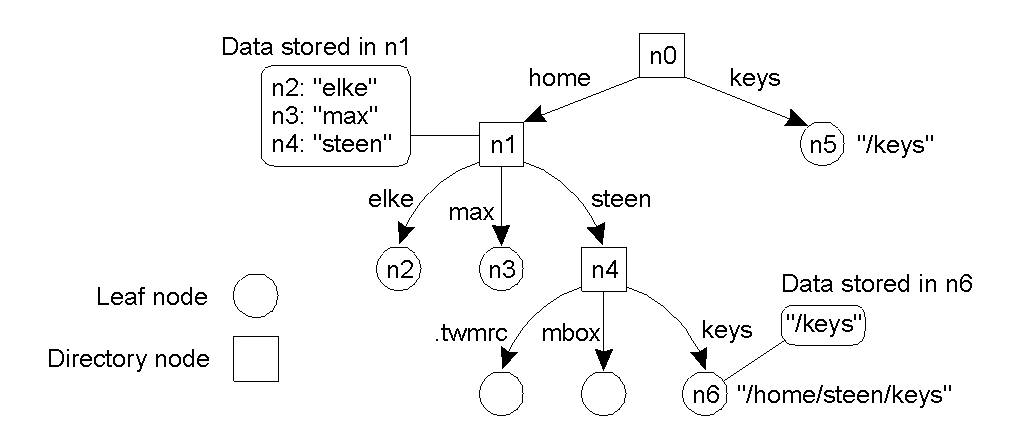
\includegraphics[scale=0.5]{img/symboliclink.png}
\caption{Esempio di hard link}\label{img:symboliclink}
\end{figure}
\subsubsection{Implementazione di uno spazio dei nomi}
Lo spazio dei nomi come abbiamo visto è il cuore di un \emph{naming service}. Un naming service è implementato da un name server. Se un sistema distribuito è limitato ad una rete locale è possibile implementare un name service mediante un unico name server centralizzato. Se invece il sistema ha molte entità ed è distribuito su larga scala allora è necessario distribuire il name server su più macchine.
\paragraph{Distribuzione dello spazio dei nomi}
Gli spazi dei nomi per sistemi distribuiti su larga scala sono solitamente organizzati gerarchicamente. Il \textbf{livello globale} è costituito dai nomi di più alto livello cioè il nodo radice ed i nodi directory logicamente più vicini ad essa. i nodi del livello globale sono spesso caratterizzati per la loro stabilità nel senso che le directory table cambiano raramente. Tali nodi possono rappresentare le aziende o i gruppi di aziende i cui nomi sono memorizzati nello spazio dei nomi.\\
Il \textbf{livello amministrativo} è costituito dai nodi directory gestiti da una sola azienda, questi nodi rappresentano gruppi di entità che appartengono alla stessa azienda o unità amministrativa, come un nodo per ogni per ogni dipartimento dell'azienda oppure uno utilizzato solo per gli utenti.\\
Il \textbf{livello gestionale} è il livello più basso ed è costituito da nodi che cambiano regolarmente. A questo gruppo appartengono gli host di una rete interna. Diversamente dagli altri livelli questi host sono gestiti non solo dagli amministratori ma anche dagli utenti finali.\\
La \figurename\,\ref{img:dnslevel} mostra una possibile suddivisione dello spazio dei nomi del DNS. Lo spazio dei nomi è diviso in parti non sovrapponibili chiamate \textbf{zone}. Una zona è uno spazio dei nomi che è implementato da un nameserver separato.
\begin{figure}
\centering
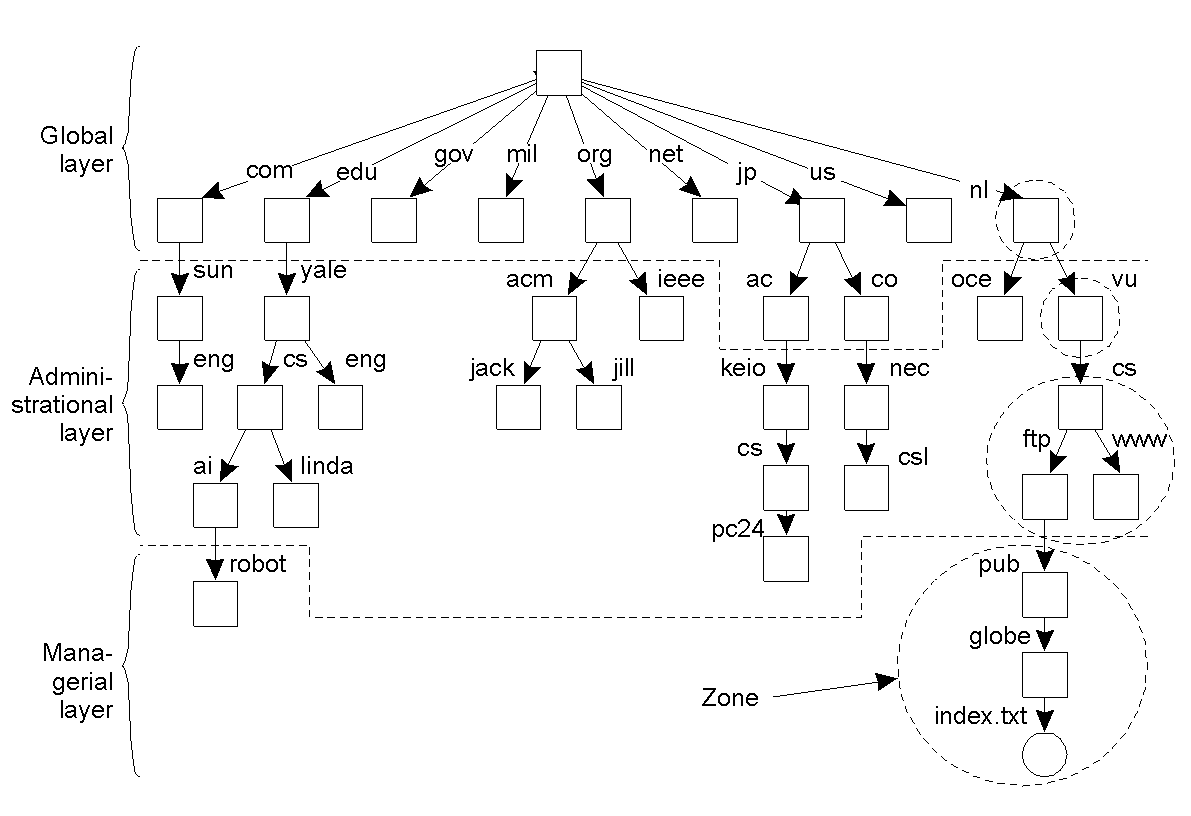
\includegraphics[scale=0.5]{img/dnslevel.png}
\caption{Esempio di suddivisione dei tre livelli nello spazio dei nomi del DNS}\label{img:dnslevel}
\end{figure}
Relativamente a disponibilità e prestazioni i name server dei diversi livelli devono rispettare diversi requisiti. I name server del livello globale devono essere altamente disponibili, in quanto se un name server si guasta un'ampia parte dello spazio dei nomi diventa irraggiungibile. Per quanto riguarda le prestazioni invece sono un po meno critiche in quanto cambiando raramente i risultati di ricerca possono essere memorizzati localmente dai client tramite meccanismi di cache. Il \emph{throughtput} però deve essere elevato in quanto le richieste provengono da una grande quantità di utenti. I requisiti di disponibilità e di prestazzioni per i server di livello globale possono essere soddisfatti replicando i server in combinazione con i meccanismi di cache.\\
La disponibilità dei name server a livello amministrativo è importante per i client all'interno della stessa azienda, infatti se si guasta le risorse all'interno dell'azienda diventano irraggiungibili. In merito alle prestazioni sono molto simili a quelle del livello globale in quanto anche qui i nodi non cambiano spesso, tuttavia, le tempistiche per i risultati delle ricerche devono essere nell'ordine di qualche millisecondo, anche gli aggiornamenti devono essere tempestivi, infatti, è inaccettabile che per l'attivazione di un account si debba aspettare qualche ora.\\
I requisiti prestazionali dei name server a livello gestionale sono molto più stringenti, la disponibilità non è importante ma le prestazioni sono una caratteristica molto importante in quanto gli utenti si aspettano che le operazioni avvengano immediatamente. Inoltre a causa dei continui aggiornamenti i meccanismi di cache lato client non sono efficaci e bisogna perciò interrogare sempre il nameserver.
\paragraph{Implementazione dello spazio dei nomi}
La distribuzione di uno spazio dei nomi su più \emph{name server} influenza l'implementazione della risoluzione dei nomi. Per spiegare la loro implemnetazione partiamo perciò dal caso più semplice in cui i name server non siano replicati ne che abbiano meccanismi di cache.\\
Ogni client ha accesso ad un \textbf{name resolver} locale responsabile di portare avanti il processo di risoluzione dei nomi. Partiamo dall'esempio mostrato anche in \figurename\,\ref{img:dnslevel} e focalizziamoci sulla risoluzione del \emph{path name} assoluto:
$$root:<nl,vu,cs,ftp,pub,globe,index.html>$$
che usando una notazione URL è possibile tradurre in \emph{ftp://ftp.cs.vu.nl/pub/globe/index.html}.\\
Esisstono due modi per implementare la risoluzione dei nomi. Il primo metodo è quello della \textbf{risoluzione dei nomi iterativa}, un \emph{name resolver} passa ak \emph{root name server} il nome completo . Il \emph{root server} risolverà il nome appena possibile e lo restituirà al client, nel nostro esempio il \emph{root server} può risolvere solo l'etichetta \emph{nl} per la quale restituirà l'indirizzo del name server associato. A questo punto il client passa il resto del path name (cioè $nl:<vu,cs,ftp,pub,globe,index.html>$) a quel name server. Questo server può risolvere solo l'etichetta \emph{vu} e restituisce l'indirizzo del name server associato. Il \emph{name resolver} continuerà così fino alla completa risoluzione del nome. Questo processo è mostrato in \figurename\,\ref{img:iterativa} dove la notazione $\#<cs>$ indica l'indirizzo del server che si occupa della parte \emph{cs} del nome.\\
\begin{figure}[htb]
\centering
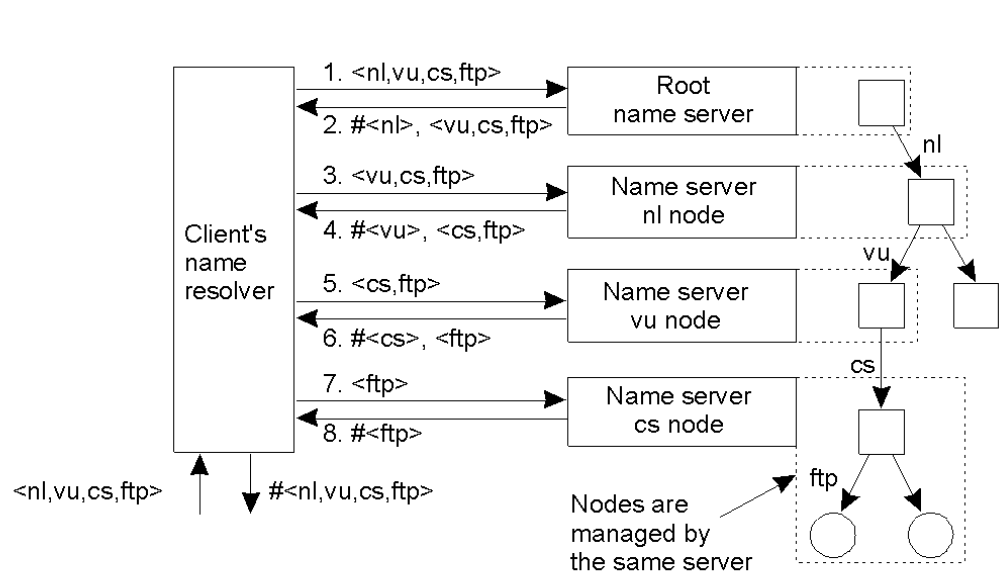
\includegraphics[scale=0.45]{img/iterativa.png}
\caption{Risoluzione dei nomi iterativa}\label{img:iterativa}
\end{figure}
In alternativa al meccanismo iterativo è possibile usare la ricorsione, invece di restituire ogni risultato intermedio al client un \emph{name server} passa il risultato al name server successivo. Questo meccanismo mostrato in \figurename\,\ref{img:ricorsiva} è chiamato \textbf{risoluzione dei nomi ricorsiva.} In questo caso quando il root name server trova l'indirizzo del server che implementa il nodo chiamato \emph{nl} gli chiede di risolvere il path $nl:<vu,cs,ftp,pub,globe,index.html>$, il quale a sua volta individuerà il server che implementa \emph{vu} e gli chiederà di risolvere il rimanente path.\\
L'inconveniente di questo tipo di risoluzione è che richiede ai name server livelli prestazionali maggiori rispetto alla versione iterativa.
\begin{figure}[htb]
\centering
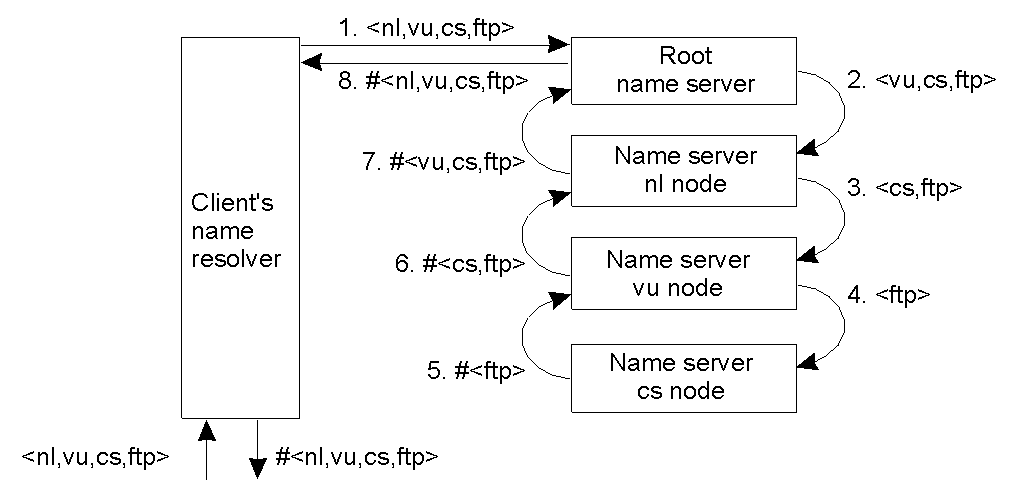
\includegraphics[scale=0.45]{img/ricorsiva.png}
\caption{Risoluzione dei nomi ricorsiva}\label{img:ricorsiva}
\end{figure}
Tuttavia l'approccio ricorsivo presenta anche alcuni vantaggi, ad esempio, il cacheing è molto più efficace rispetto al caso iterativo inoltre, i costi di comunicazione sono ridotti al minimo.
\subsubsection{DNS}
Uno dei servizi di \emph{naming} più diffusi oggi al mondo è il \emph{domain name system} (DNS) di Internet. Il DNS è principalmente usato per ricercare gli indirizzi IP degli host e dei mail server. 
\paragraph{Spazio dei nomi del DNS}
Lo spazio dei nomi del DNS è organizzato gerarchicamente come un albero con radice.
Un'etichetta è una stringa \emph{case insensitive} costituita da caratteri alfanumerici con una lunghezza massima di 63 caratteri; la lunghezza di un path è limitata a 255 caratteri. La rappresentazione di un path name in forma di stringa parte dall'etichetta più a destra e separata da un punto ("."). Anche la radice è rappresentata da un punto ma questo di solito viene omesso. Un esempio è il path name $root:<nl,vu,cs,flits>$ che rappresentato sotto forma di stringa diventa \emph{flits.cs.vu.nl}.\\
Dato che un nodo nello spazio dei nodi ha esattamente un arco in entrata la sua etichetta viene usata come nome del nodo. Un sottoalbero è chiamato \textbf{dominio} ed il path name verso il suo nodo radice è chiamato \textbf{nome del dominio.} Il contenuto di un nodo è costituito da un insieme di \textbf{resource record} i quali possono essere di diverso tipo e sono illustrati in \tablename\,\ref{tab:resource}.
\begin{table}
\centering
\begin{tabular}{|l|l|p{0.5\textwidth}|}
\hline
\textbf{Tipo di record} & \textbf{Entità associata} & \textbf{Descrizone} \\
\hline
SOA & Zona & Informazioni sulla zona rappresentata \\
A & Host & Contiene un indirizzo IP dell'host che questo nodo rappresenta \\
MX & Dominio & Si riferisce ad un mail server che gestisce le mail indirizzate a questo nodo \\
SRV & Dominio & Si riferisce ad un server che gestisce un particolare servizio \\
NS & Zona & Indica il name server che implementa la zona rappresentata \\
CNAME & Nodo & Link simbolico con il nome primario del nodo rappresentato \\
PTR & Host & Contiene il nome canonico dell'host \\
HINFO & Host & Mantiene informazioni sull'host che questo nodo rappresenta \\
TXT & Qualunque tipo & Contiene qualunque tipo di informazione \\
\hline
\end{tabular}
\caption{Tipi importanti di resource record}\label{tab:resource}
\end{table}
Analiziamo ora alcuni campi dei resource record; un campo SOA contiene informazioni quali l'indirizzo mail dell'amministratore di sistema, il nome dell'host dal quale prelevare informazioni sulla zona ecc.
Il resource A(\emph{address}) rappresenta un particolare host in internet, il campo A contiene il suo indirizzo IP, in caso di host \emph{multihomed} un nodo conterrà più campi A.
I record MX (\emph{mail exchange}) sono contengono un link simbolico a un nodo che rappresenta il mail server per quella zona.\\
Un esempio di tali record sono rappresentati in \figurename\,\ref{img:resourcer}
\begin{figure}[htb]
\centering
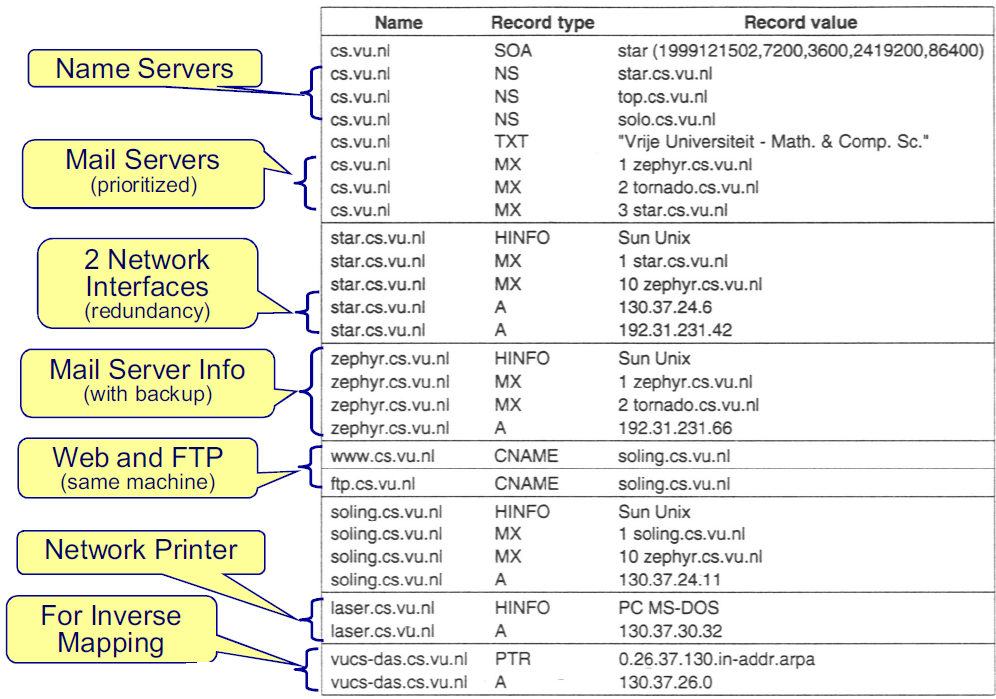
\includegraphics[scale=0.5]{img/resourcer.png}
\caption{Esempio di resource record estratto dalla base di dati per la zona \emph{cs.vu.nl}}\label{img:resourcer}
\end{figure}
\paragraph{Implementazione del DNS}
In sostanza , lo spazio dei nomi del DNS è suddivisibile in un livello globale ed uno amministrativo come mostrato in \figurename\,\ref{img:dnslevel}. Il livello gestionale solitamente è gestito a livello locale e quindi non fa parte del DNS. Ogni zona è implementata da un name server replicato per garantirne la disponibilità. Gli aggiornamenti della zona sono solitamente gestiti dal server primario. Gli aggiornamenti vengono propagati ai server secondari solo tramite richiesta di quest'ultimi, questo procedimento è chiamato \textbf{trasferimento di zona}.\\
Una base di dati del DNS è un insieme di file contenete diversi \emph{resource record} tra questi file uno in particolare contiene gli identificatori di tutti i nodi di una particolare zona in modo da consentire l'identificazione di tutti i nodi semplicemente mediante il nome del loro dominio.
\subsection{Naming basato sugli attributi}
I nomi semplici e quelli strutturati offrono la possibilità di far riferimento ad un'entità in modo indipendente dalla sua posizione. Inoltre i nomi strutturati sono progettati per essere relativamente \emph{human-friendly}. Ma a volte non interessa il nome dell'entità ma un utente vorrebbe ricercare una risorsa in base ad una serie di attributi specificati.\\
Un modo assai diffuso per effettuare questa ricerca è usare un sistema di \textbf{naming basato sugli attributi}, il quale consiste nel descrivere un'entità in termini di coppie (\emph{attributo, valore}) e ad ogni entità possono essere associati più attributi diversi.
\subsubsection{Directory service}
I sistemi di naming basati sugli attributi sono anche conosciuti come \textbf{directory service}. Con questo meccanismo le entità hanno associato un insieme di attributi utilizzabili per le ricerche. Ad esempio in un sistema di mail i messaggi possono essere etichettati tramite attributi relativi al mittente al destinatario all'oggetto e così via; quando però si vuole ampliare il meccanismo dei descrittori risulta un po più difficile, in quanto la maggior parte delle volte tale meccanismo viene impostato manualmente.\\
Per attenuare alcune problematiche sono state introdotti diversi framework tra cui il \textbf{resource description framework} (\textbf{RDF}) il quale basa la sua descrizione su una tripletta formata da soggetto, predicato e oggetto i quali possono essere delle risorse oltre che degli attributi come nel caso della tripletta (\emph{Persona, nome, Alice}) dove si fa riferimento ad una risorsa di tipo \emph{Persona} il cui \emph{nome} è \emph{Alice}.\\
A differenza dei sistemi di naming strutturati la ricerca dei valori in un sistema di naming basato sugli attributi richiede di effettuare una ricerca esaustiva su tutti i descrittori.
\subsubsection{LDAP}
Un approccio diffuso di affrontare il problema dei directory service è quello di combinare il naming strutturato con quello basato sugli attributi, questo approccio è stato ampiamente usato nel servizio \emph{Active Directory} di Microsoft ed in altri sistemi. Molti di questi sistemi utilizzano o si basano sul \textbf{light directory access protocol} comunemente chiamato anche \textbf{LDAP}.\\
Un directory service LDAP consiste in un certo numero di record di solito chiamati elementi della directory. Un elemento della directory è paragonabile ad un resource record del DNS. Ogni record è composto da una coppia (\emph{attributo, valore}) in cui ogni attributo ha un tipo associato. L'insieme di tutti gli elementi di un directory service LDAP è chamato \textbf{directory information base} (\textbf{DIB}). Un aspetto importante di un DIB è che ogni record ha un nome univoco in modo da renderlo identificabile, tale nome appare in ogni record come la sequenza di attributi di naming. Ogni attributo di naming è chiamato \textbf{relative distinguished name} o in breve \textbf{RDN}. Come nel caso dei nomi univoci strutturati l'uso dei nomi globali ottenuti tramite l'elenco degli RDN in sequenza genera una gerarchia degli elemnti della directory chiamata anche \textbf{directory information tree} (\textbf{DIT}). Un DIT non è altro che un grafo dei nomi in un sistema basato su LDAP in cui ogni nodo è un elemento della directory. In tal senso alcuni nodi possono agire sia da elemento sia da directory nel senso tradizionale del termine. Per accedere a tali elementi possiamo utilizzare due distinte  funzioni di interrogazione, la \texttt{read} che è utilizzata per leggere il contenuto di un elemento, e la \texttt{list} utilizzata per elencare i diversi archi in uscita come mostrato in \figurename\,\ref{fig:readlist}.
\begin{figure}[hbt]
\subfigure[]{
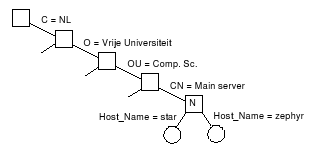
\includegraphics[width=7.5cm]{img/dit.png}
\label{fig:dit}
}
\subfigure[]{
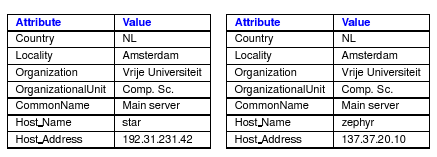
\includegraphics[width=7.5cm]{img/readlist.png}
\label{fig:readlist}
}
\caption{Esempio di DIT \ref{fig:dit} e di valori restituiti da un operazione di list e di read \ref{fig:readlist}}
\end{figure}
Quando si ha progetta un sistema basato su LDAP di larga scala il DIT viene suddiviso su più server chiamati \textbf{directory server agent (DSA)} mentre i client sono chiamati \textbf{directory user agent} o DUA i quali sono simili ai name resolver nel sistema DNS.
\subsection{Removing}
I sistemi di naming fin qui descritti permettono l'accesso a delle entità distribuite molte volte in maniera globale. Ma quando queste entità non vengono più referenziate devono essere eliminate, per fare ciò solitamente si utilizza un garbage collector ma in un ambiente distribuito le cose si complicano alquanto.\\
Esistono tuttavia diversi meccanismi per capire se un entità è ancora differenziata.
\subsubsection{Reference counting}
In questo meccanismo gli oggetti tengono conto di quanti altri oggetti possiedono un loro riferimento, il sistema risulta molto efficiente se il conteggio è fatto tramite l'invio di un solo messaggio come mostrato in \figurename\,\ref{fig:referencecounting} (a) ma purtroppo si potrebbero verificare dei problemi di \emph{race condition} quando si passano dei riferimenti tra processi. Una tecnica è quella di comunicare all'oggetto anche il passaggio di riferimento ad altri processi come mostrato in \figurename\,\ref{fig:referencecounting} (b) questo meccanismoo purtroppo degrada le prestazioni in quanto i messaggi scambianti diventano tre.\\
\begin{figure}[htb]
\centering
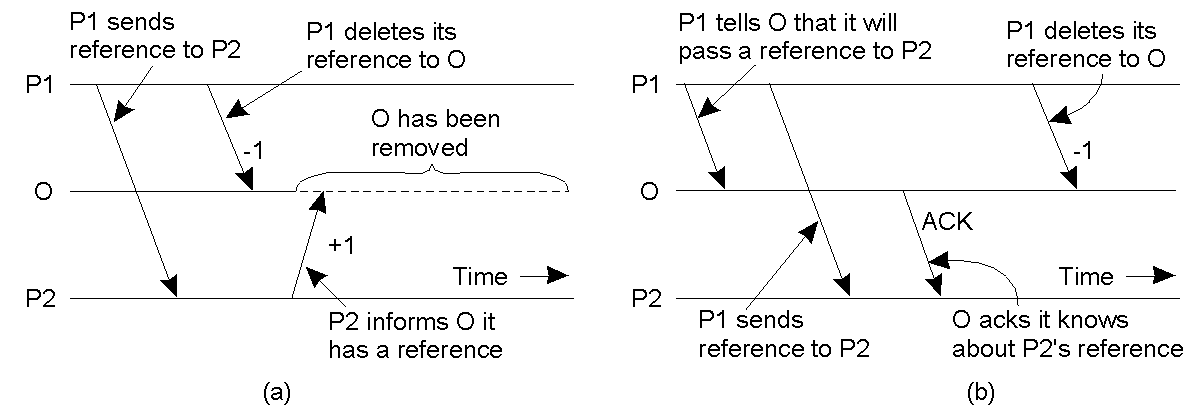
\includegraphics[scale=0.4]{img/referencecounting.png}
\caption{Esempio di reference counting con lo scambio di uno (a) e tre (b) messaggi}\label{fig:referencecounting}
\end{figure}
Un meccanismo simile ma che evita la race condition è quello che utilizza dei pesi per gli oggetti e comunica soltanto il decremento di tali pesi come mostrato in \figurename\,\ref{fig:weight} dove il peso di un oggetto viene diviso tra i due processi che usano tale oggetto, in questo caso al processo $P_2$ il riferimento viene passato dal processo $P_1$. Quando il peso totale e il peso dell'oggetto tornano a pareggiarsi l'oggeto può essere rimosso in quanto non più referenziato. 
\begin{figure}[htb]
\centering
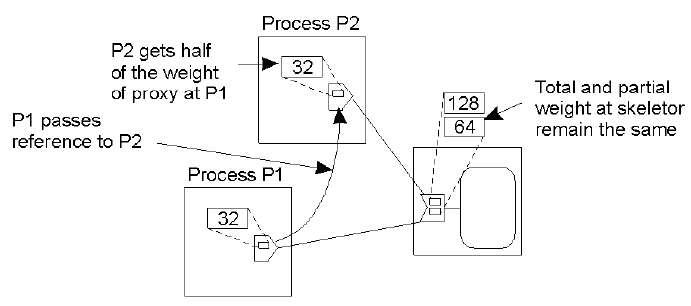
\includegraphics[scale=0.6]{img/weight.png}
\caption{Esempio di reference counting con il meccanismo dei pesi}\label{fig:weight}
\end{figure}
Il problema di questa tecnica è che sono possibili solo un numero limitato di riferimenti. La soluzione è quella di concatenare i riferimenti come mostrato in \figurename\,\ref{fig:weightconcat}; questo risolve il problema dei riferimenti limitati ma aggiunge un hop per l'accesso all'oggetto.
\begin{figure}[htb]
\centering
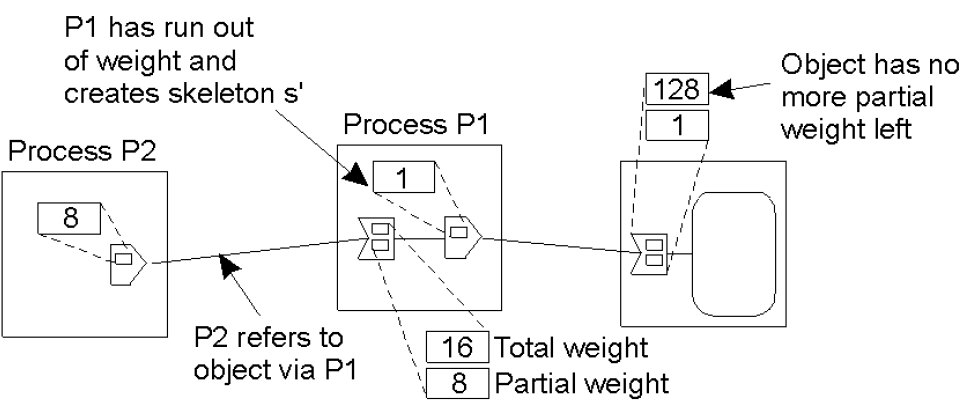
\includegraphics[scale=0.4]{img/weightconcat.png}
\caption{Esempio di reference counting con il meccanismo dei pesi e la concatenazione}\label{fig:weightconcat}
\end{figure}
\subsubsection{Reference listing}
Un altro meccanismo molto utilizzato è quello del reference listing che non tiene traccia del numero di referenze ma soltanto dell'identità di chi richiede un riferimento, il vantaggio è che l'inserimento o l'eliminazione di un proxy (inteso come processo che richiede il riferimento) è idempotente ovvero inserimento e cancellazione di un proxy richiedono un messaggio di ack ma le richieste multiple non hanno effetto sul carico di rete. Il secondo vantaggio è che le risorse orfane possono essere individuate facilmente pingando periodicamente i client presenti nella lista dei riferimenti. Tuttavia anche questo meccanismo soffre del fenomento di race condition quando viene copiato un riferimento.
\subsubsection{Distributed mark-and-sweep}
Il mark and sweep permette di tenere traccia di quelle entità orfane. Nel caso di sistema uniprocessore tale meccanismo si suddivide in due fasi, nella prima fase vengono marchiate tutte le entità accessibili da qualche tipo di referenza. Tutti i nodi partono colorati di bianco, un nodo viene colorato di grigio quando è possibile raggiungerlo dalla root ma alcune delle sue referenze non sono ancora state valutate, infine viene marcato di nero se tutte le sue referenze sono marchiate di grigio.\\
Nella seconda fase il garbage collector elimina tutti i nodi marchiati di bianco.\\
Nel caso di sistema distribuito il garbage collector entra in funzione su ogni nodo, partendo da un nodo P una risorsa viene marchiata di grigio se è possibile raggiungerla dalla root del nodo P quando un proxy $q$ è marchiato di grigio si invia un messaggio a tutti i suoi riferimenti. Quando tutti i riferimenti rispondono con un ack il proxy $q$ viene marchiato di nero.
\section{Sincronizzazione}
\subsection{Sincronizzazione nei sistemi distribuiti}
\subsection{Sincronizzazione dei clock}
\subsubsection{Orologi fisici}
\subsubsection{Global positioning system}
\subsubsection{Algoritmi di sincronizzazione dei clock}
\subsection{Orologi logici}
\subsubsection{Clock scalari}
\subsubsection{Clock vettoriali}
\subsection{Mutua esclusione}
\subsubsection{Panoramica}
\subsubsection{Un algoritmo centralizzato}
\subsubsection{Un algoritmo decentralizzato}
\subsubsection{Un algoritmo distribuito}
\subsubsection{Un algoritmo token ring}
\subsubsection{Confronto tra algoritmi}
\subsection{Algoritmi di elezione}
\subsubsection{Algoritmo di elezione tradizionale}
\subsubsection{Algoritmo di elezione token ring}
\subsection{Collection global state}
\subsubsection{Termination detection}
\subsection{Transizioni distribuite}
\subsubsection{Individuazione di deadlock distribuiti}
\section{Tolleranza ai guasti}\label{capitolo8}
\subsection{Introduzione alla tolleranza ai guasti}
\subsubsection{Concetti base}
\subsubsection{Modelli di guasto}
\subsubsection{La ridondanza}
\subsection{Comunicazione client server affidabile}
\subsubsection{Comunicazione punto-a-punto}
\subsubsection{RPC in presenza di fallimenti}
\subsection{Protezione contro i fallimenti}
\subsubsection{Elementi di progettazione}
\subsubsection{Mascheramento dei guasti e meccanismi di replica}
\subsubsection{Accordo nei sistemi guasti}
\subsubsection{Rilevamento dei guasti}
\subsection{Comunicazione affidabile nei gruppi}
\subsubsection{Multicasting affidabile}
\subsubsection{Scalabilità del multicasting affidabile}
\subsubsection{Multicasting atomico}
\subsection{Commit distribuiti}
\subsubsection{Commit a due fasi}
\subsubsection{Commit a tre fasi}
\subsection{Tecniche di ripstistino}
\subsubsection{Introduzione}
\subsubsection{Creazione di checkpoint}
\subsubsection{Logging dei messaggi}

\end{document}